%%%%%%%%%%%%%%%%%%%%%%%%%%%%%%%%%%%
%This is the LaTeX ARTICLE template for RSC journals
%Copyright The Royal Society of Chemistry 2016
%%%%%%%%%%%%%%%%%%%%%%%%%%%%%%%%%%%

\documentclass[twoside,twocolumn,9pt]{article}
\usepackage{extsizes}
\usepackage[super,sort&compress,comma]{natbib} 
\usepackage[version=3]{mhchem}
\usepackage[left=1.5cm, right=1.5cm, top=1.785cm, bottom=2.0cm]{geometry}
\usepackage{balance}
\usepackage{mathptmx}
\usepackage{sectsty}
\usepackage{graphicx}
\usepackage{lastpage}
\usepackage[format=plain,justification=justified,singlelinecheck=false,font={stretch=1.125,small,sf},labelfont=bf,labelsep=space]{caption}
\usepackage{float}
\usepackage{fancyhdr}
\usepackage{fnpos}
\usepackage[english]{babel}
\addto{\captionsenglish}{%
  \renewcommand{\refname}{Notes and references}
}
\usepackage{array}
\usepackage{droidsans}
\usepackage{charter}
\usepackage[T1]{fontenc}
\usepackage[usenames,dvipsnames]{xcolor}
\usepackage{setspace}
\usepackage[compact]{titlesec}
\usepackage{hyperref}
\usepackage[utf8]{inputenc} % input encoding
\usepackage{lmodern}
%%%Please don't disable any packages in the preamble, as this may cause the template to display incorrectly.%%%

\usepackage{epstopdf}%This line makes .eps figures into .pdf - please comment out if not required.

\definecolor{cream}{RGB}{222,217,201}

\begin{document}

\pagestyle{fancy}
\thispagestyle{plain}
\fancypagestyle{plain}{
%%%HEADER%%%
\renewcommand{\headrulewidth}{0pt}
}
%%%END OF HEADER%%%

%%%PAGE SETUP - Please do not change any commands within this section%%%
\makeFNbottom
\makeatletter
\renewcommand\LARGE{\@setfontsize\LARGE{15pt}{17}}
\renewcommand\Large{\@setfontsize\Large{12pt}{14}}
\renewcommand\large{\@setfontsize\large{10pt}{12}}
\renewcommand\footnotesize{\@setfontsize\footnotesize{7pt}{10}}
\makeatother

\renewcommand{\thefootnote}{\fnsymbol{footnote}}
\renewcommand\footnoterule{\vspace*{1pt}% 
\color{cream}\hrule width 3.5in height 0.4pt \color{black}\vspace*{5pt}} 
\setcounter{secnumdepth}{5}

\makeatletter 
\renewcommand\@biblabel[1]{#1}            
\renewcommand\@makefntext[1]% 
{\noindent\makebox[0pt][r]{\@thefnmark\,}#1}
\makeatother 
\renewcommand{\figurename}{\small{Fig.}~}
\sectionfont{\sffamily\Large}
\subsectionfont{\normalsize}
\subsubsectionfont{\bf}
\setstretch{1.125} %In particular, please do not alter this line.
\setlength{\skip\footins}{0.8cm}
\setlength{\footnotesep}{0.25cm}
\setlength{\jot}{10pt}
\titlespacing*{\section}{0pt}{4pt}{4pt}
\titlespacing*{\subsection}{0pt}{15pt}{1pt}
%%%END OF PAGE SETUP%%%

%%%FOOTER%%%
\fancyfoot{}
\fancyfoot[LO,RE]{\vspace{-7.1pt}\includegraphics[height=9pt]{head_foot/LF}}
\fancyfoot[CO]{\vspace{-7.1pt}\hspace{11.9cm}\includegraphics{head_foot/RF}}
\fancyfoot[CE]{\vspace{-7.2pt}\hspace{-13.2cm}\includegraphics{head_foot/RF}}
\fancyfoot[RO]{\footnotesize{\sffamily{1--\pageref{LastPage} ~\textbar  \hspace{2pt}\thepage}}}
\fancyfoot[LE]{\footnotesize{\sffamily{\thepage~\textbar\hspace{4.65cm} 1--\pageref{LastPage}}}}
\fancyhead{}
\renewcommand{\headrulewidth}{0pt} 
\renewcommand{\footrulewidth}{0pt}
\setlength{\arrayrulewidth}{1pt}
\setlength{\columnsep}{6.5mm}
\setlength\bibsep{1pt}
%%%END OF FOOTER%%%

%%%FIGURE SETUP - please do not change any commands within this section%%%
\makeatletter 
\newlength{\figrulesep} 
\setlength{\figrulesep}{0.5\textfloatsep} 

\newcommand{\topfigrule}{\vspace*{-1pt}% 
\noindent{\color{cream}\rule[-\figrulesep]{\columnwidth}{1.5pt}} }

\newcommand{\botfigrule}{\vspace*{-2pt}% 
\noindent{\color{cream}\rule[\figrulesep]{\columnwidth}{1.5pt}} }

\newcommand{\dblfigrule}{\vspace*{-1pt}% 
\noindent{\color{cream}\rule[-\figrulesep]{\textwidth}{1.5pt}} }

\makeatother
%%%END OF FIGURE SETUP%%%

%%%TITLE, AUTHORS AND ABSTRACT%%%
\twocolumn[
  \begin{@twocolumnfalse}
{\includegraphics[height=30pt]{head_foot/PCCP}\hfill\raisebox{0pt}[0pt][0pt]{\includegraphics[height=55pt]{head_foot/RSC_LOGO_CMYK}}\\[1ex]
\includegraphics[width=18.5cm]{head_foot/header_bar}}\par
\vspace{1em}
\sffamily
\begin{tabular}{m{4.5cm} p{13.5cm}}

\includegraphics{head_foot/DOI} & \noindent\LARGE{\textbf{Spin-dependent transport and spin transfer torque in a borophene-based spin valve$^\dag$}} \\%Article title goes here instead of the text "This is the title"
&\noindent\large{Erfan Nikan,$^{\ast}$\textit{$^{a}$} Amirhossein Ahmadkhan Kordbacheh,\textit{$^{b\ddag}$}} \\%Author names go here instead of "Full name", etc.

\includegraphics{head_foot/dates} & \noindent\normalsize{This article presents a theoretical analysis of spin-dependent transport and spin-transport torque for a borophene-based ferromagnetic/normal/ferromagnetic junction. This study focuses on borophene nanoribbons (BNRs) as a basis for spin valve numerical calculations for conduction in both configurations where the magnetization vectors of the leads are parallel or antiparallel to each other (P and AP configurations, respectively), magnetoresistance (MR), and spin transfer torque (STT). The Landauer formalism and non-equilibrium Green's function (NEGF) approaches are used to derive the spin-dependent tunneling currents in the Magnetic Tunnel Junction (MTJ). The results of the calculations for a Zigzag BNR show that the conductance is always larger than $e^2/h$ for the P configuration of lead magnetizations. For the AP configuration, the conductance becomes zero in specific energy ranges. A perfect MR plateau is found for the junction in the absence of disorder, which proves to be an excellent spin valve candidate. The variations of STT with Fermi energy, the relative angle between two electrode magnetizations, are studied for different strengths of ferromagnetic magnetization. The STT per unit bias voltage, as a function of Fermi energy, decreases significantly in the Dirac point energy. A sinusoidal oscillatory pattern can be evidently observed in the STT at unit bias voltage $V$ versus the angle between the magnetizations of two electrodes, which amplifies as M increases. Borophene has unique properties, including low density and high hardness, heat resistance, and electrical conductance, which make it a promising candidate for spintronic. The article provides a comprehensive analysis of the spin-dependent properties of borophene and its potential applications in spintronics.} \\%The abstrast goes here instead of the text "The abstract should be..."

\end{tabular}
\end{@twocolumnfalse} \vspace{0.6cm}
%%%END OF TITLE, AUTHORS AND ABSTRACT%%%
]
%%%FONT SETUP - please do not change any commands within this section
\renewcommand*\rmdefault{bch}\normalfont\upshape
\rmfamily
\section*{I}
\vspace{-1cm}

%%%FOOTNOTES%%%
\footnotetext{\textit{$^{a}$~Materials Simulation Laboratory, Department of Physics, Iran University of Science and Technology, Tehran 1684613114, Iran.E-mail:nikan\textunderscore{}er96@physics.iust.ac.ir}}
\footnotetext{\textit{$^{b}$~Materials Simulation Laboratory, Department of Physics, Iran University of Science and Technology, Tehran 1684613114, Iran.E-mail:akordbacheh@iust.ac.ir}}
%%%END OF FOOTNOTES%%%

%%%MAIN TEXT%%%%
\section{Introduction}
Over time, Moore's law will face more serious challenges to remain effective. Due to the fact that traditional electronics are based only on the transportation and storage of electric charge, the continuation of the miniaturization process will involve more limitations and more profound challenges. Therefore, devices based on new principles have become a hotspot in the post-Moore era\cite{zhu2023recent,zhou2020defect}. 

Spintronics is one of the technologies that may defy Moore's law. The goal of spintronics is to understand the interaction of the spin of particles with the solid environment around them, especially the effect of electron spin on conductance (or current). The main problem in spintronics is the manufacturing of spintronic-based devices. Since the discovery of GMR in 1988\cite{baibich1988giant, binasch1989enhanced}, spintronics, including STT\cite{zutic2004spintronics,fert2008nobel}, semiconductor spintronics, single-electron spintronics, etc., have been active as a new research field. One of the most amazing applications of Spintronic is the spin valve effect\cite{zutic2004spintronics}, which can be manipulated by the relative angle of magnetizations of the magnetic layers in the leads. 

The spin valve was first developed in 1991\cite{dieny1991giant}, which later revolutionized the industry of magnetic sensors, hard disk heads, and magnetic random access memories (MRAM)\cite{heim1994design,freitas1994spin,leal1994unshielded,tsang1994design}. The spin valve device consists of two or more magnetic connections. In a spin valve device with two magnetic connections, depending on whether the magnetic connections are in the direction of in-plane flow (CIP) or perpendicular to the plane (CPP), two different geometrical structures are formed. Magnetic resistance refers to the phenomenon that the resistance of a metal or semiconductor changes with an external magnetic field. The MR effect can be analyzed using a spin valve device\cite{bandyopadhyay2008introduction}. Depending on whether the sandwiched channel in the spin valve is metallic or insulating, the phenomenon of magnetoresistance (GMR) and tunnel magnetoresistance (TMR) can be observed\cite{fong2016spin}. In addition to describing the physics behind MR behavior, the theoretical investigation of MR also studies the role of various effective parameters in MR behavior\cite{harikumar2020non}.

Spin transfer torque (STT) has attracted the attention of many researchers due to the use of electron spin in storage technology and sensors\cite{liu2013spin}. Ralph and Stiles theoretically presented the physics of STT in magnetic devices\cite{ralph2008spin}. Abert et al. investigated STT using the spin-diffusion model\cite{abert2017field}, and Zhang et al. examined the magnetic switching mechanism by including the exchange interaction\cite{zhang2002mechanisms}.

\begin{figure*}
\resizebox{0.95\textwidth}{!}{\includegraphics{Shematic3.png}}
\caption{Schematically shows the structure of a $\beta$-borophene-based spin valve with magnetic leads, where the magnetization vectors of the two leads can have a relative angle $\theta$. The magnetization of the leads is caused by the magnetic substrate on which they are placed, which can be experimentally controlled. In the upper part of the figure, a nanoribbon borophene with armchair edges is illustrated, and in the lower part of the figure, a zigzag borophene nanoribbon is depicted. The borophene unit cell with boron atoms labeled in a zigzag-edge borophene is shown in Table\ref{tbl:hopping}, where the on-site energies and hopping parameters of the atoms are given.
}
\label{fig:model}
\end{figure*}

\begin{figure*}[ht]
    \centering
    \resizebox{0.45\textwidth}{!}{\input{Armchair-Antiparallel-conductance-revise.tex}}
    \resizebox{0.45\textwidth}{!}{% GNUPLOT: LaTeX picture with Postscript
\begin{latin}
\begingroup
  % Encoding inside the plot.  In the header of your document, this encoding
  % should to defined, e.g., by using
  % \usepackage[cp1252,<other encodings>]{inputenc}
  % \inputencoding{cp1252}%
  \makeatletter
  \providecommand\color[2][]{%
    \GenericError{(gnuplot) \space\space\space\@spaces}{%
      Package color not loaded in conjunction with
      terminal option `colourtext'%
    }{See the gnuplot documentation for explanation.%
    }{Either use 'blacktext' in gnuplot or load the package
      color.sty in LaTeX.}%
    \renewcommand\color[2][]{}%
  }%
  \providecommand\includegraphics[2][]{%
    \GenericError{(gnuplot) \space\space\space\@spaces}{%
      Package graphicx or graphics not loaded%
    }{See the gnuplot documentation for explanation.%
    }{The gnuplot epslatex terminal needs graphicx.sty or graphics.sty.}%
    \renewcommand\includegraphics[2][]{}%
  }%
  \providecommand\rotatebox[2]{#2}%
  \@ifundefined{ifGPcolor}{%
    \newif\ifGPcolor
    \GPcolorfalse
  }{}%
  \@ifundefined{ifGPblacktext}{%
    \newif\ifGPblacktext
    \GPblacktexttrue
  }{}%
  % define a \g@addto@macro without @ in the name:
  \let\gplgaddtomacro\g@addto@macro
  % define empty templates for all commands taking text:
  \gdef\gplbacktext{}%
  \gdef\gplfronttext{}%
  \makeatother
  \ifGPblacktext
    % no textcolor at all
    \def\colorrgb#1{}%
    \def\colorgray#1{}%
  \else
    % gray or color?
    \ifGPcolor
      \def\colorrgb#1{\color[rgb]{#1}}%
      \def\colorgray#1{\color[gray]{#1}}%
      \expandafter\def\csname LTw\endcsname{\color{white}}%
      \expandafter\def\csname LTb\endcsname{\color{black}}%
      \expandafter\def\csname LTa\endcsname{\color{black}}%
      \expandafter\def\csname LT0\endcsname{\color[rgb]{1,0,0}}%
      \expandafter\def\csname LT1\endcsname{\color[rgb]{0,1,0}}%
      \expandafter\def\csname LT2\endcsname{\color[rgb]{0,0,1}}%
      \expandafter\def\csname LT3\endcsname{\color[rgb]{1,0,1}}%
      \expandafter\def\csname LT4\endcsname{\color[rgb]{0,1,1}}%
      \expandafter\def\csname LT5\endcsname{\color[rgb]{1,1,0}}%
      \expandafter\def\csname LT6\endcsname{\color[rgb]{0,0,0}}%
      \expandafter\def\csname LT7\endcsname{\color[rgb]{1,0.3,0}}%
      \expandafter\def\csname LT8\endcsname{\color[rgb]{0.5,0.5,0.5}}%
    \else
      % gray
      \def\colorrgb#1{\color{black}}%
      \def\colorgray#1{\color[gray]{#1}}%
      \expandafter\def\csname LTw\endcsname{\color{white}}%
      \expandafter\def\csname LTb\endcsname{\color{black}}%
      \expandafter\def\csname LTa\endcsname{\color{black}}%
      \expandafter\def\csname LT0\endcsname{\color{black}}%
      \expandafter\def\csname LT1\endcsname{\color{black}}%
      \expandafter\def\csname LT2\endcsname{\color{black}}%
      \expandafter\def\csname LT3\endcsname{\color{black}}%
      \expandafter\def\csname LT4\endcsname{\color{black}}%
      \expandafter\def\csname LT5\endcsname{\color{black}}%
      \expandafter\def\csname LT6\endcsname{\color{black}}%
      \expandafter\def\csname LT7\endcsname{\color{black}}%
      \expandafter\def\csname LT8\endcsname{\color{black}}%
    \fi
  \fi
    \setlength{\unitlength}{0.0500bp}%
    \ifx\gptboxheight\undefined%
      \newlength{\gptboxheight}%
      \newlength{\gptboxwidth}%
      \newsavebox{\gptboxtext}%
    \fi%
    \setlength{\fboxrule}{0.5pt}%
    \setlength{\fboxsep}{1pt}%
\begin{picture}(7200.00,5040.00)%
    \gplgaddtomacro\gplbacktext{%
      \csname LTb\endcsname%%
      \put(900,4200){\makebox(0,0)[r]{\strut{}$B$}}%
      \put(550,704){\makebox(0,0)[r]{\strut{}$0$}}%
      \put(550,1112){\makebox(0,0)[r]{\strut{}$1$}}%
      \put(550,1521){\makebox(0,0)[r]{\strut{}$2$}}%
      \put(550,1929){\makebox(0,0)[r]{\strut{}$3$}}%
      \put(550,2337){\makebox(0,0)[r]{\strut{}$4$}}%
      \put(550,2746){\makebox(0,0)[r]{\strut{}$5$}}%
      \put(550,3154){\makebox(0,0)[r]{\strut{}$6$}}%
      \put(550,3562){\makebox(0,0)[r]{\strut{}$7$}}%
      \put(550,3971){\makebox(0,0)[r]{\strut{}$8$}}%
      \put(550,4379){\makebox(0,0)[r]{\strut{}$9$}}%
      \put(682,484){\makebox(0,0){\strut{}$-4$}}%
      \put(1447,484){\makebox(0,0){\strut{}$-3$}}%
      \put(2212,484){\makebox(0,0){\strut{}$-2$}}%
      \put(2977,484){\makebox(0,0){\strut{}$-1$}}%
      \put(3743,484){\makebox(0,0){\strut{}$0$}}%
      \put(4508,484){\makebox(0,0){\strut{}$1$}}%
      \put(5273,484){\makebox(0,0){\strut{}$2$}}%
      \put(6038,484){\makebox(0,0){\strut{}$3$}}%
      \put(6803,484){\makebox(0,0){\strut{}$4$}}%
    }%
    \gplgaddtomacro\gplfronttext{%
      \csname LTb\endcsname%%
      \put(209,2541){\rotatebox{-270}{\makebox(0,0){\strut{}$G(e^2/h)$}}}%
      \put(3742,154){\makebox(0,0){\strut{}$E(eV)$}}%
      \csname LTb\endcsname%%
      \put(2522,4206){\makebox(0,0)[r]{\strut{}$M=0$}}%
      \csname LTb\endcsname%%
      \put(2522,3986){\makebox(0,0)[r]{\strut{}$M=0.05$}}%
      \csname LTb\endcsname%%
      \put(4169,4206){\makebox(0,0)[r]{\strut{}$M=0.1$}}%
      \csname LTb\endcsname%%
      \put(4169,3986){\makebox(0,0)[r]{\strut{}$M=0.2$}}%
      \csname LTb\endcsname%%
      \put(5816,4206){\makebox(0,0)[r]{\strut{}$M=0.3$}}%
      \csname LTb\endcsname%%
      \put(3742,4709){\makebox(0,0){\strut{}Parallel}}%
    }%
    \gplbacktext
    \put(0,0){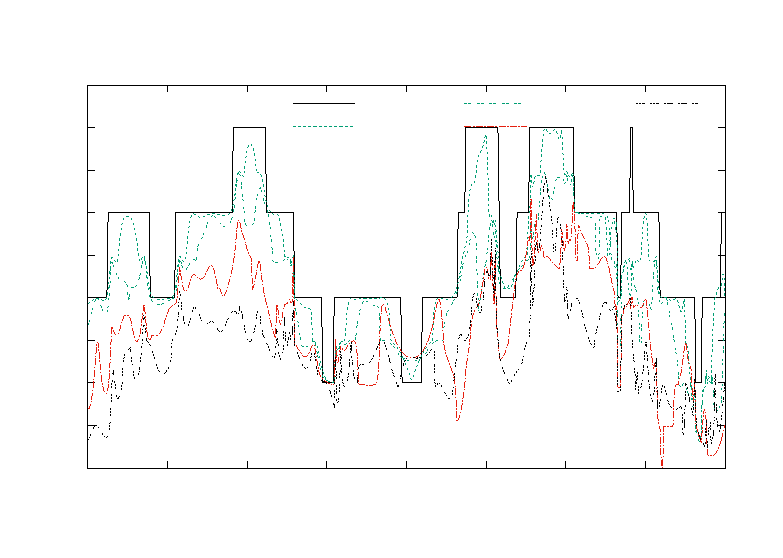
\includegraphics[width={360.00bp},height={252.00bp}]{armchair-parallel-conductance-revise}}%
    \gplfronttext
  \end{picture}%
\endgroup
\end{latin}}
    \resizebox{0.45\textwidth}{!}{% GNUPLOT: LaTeX picture with Postscript
\begingroup
  % Encoding inside the plot.  In the header of your document, this encoding
  % should to defined, e.g., by using
  % \usepackage[cp1252,<other encodings>]{inputenc}
  % \inputencoding{cp1252}%
  \makeatletter
  \providecommand\color[2][]{%
    \GenericError{(gnuplot) \space\space\space\@spaces}{%
      Package color not loaded in conjunction with
      terminal option `colourtext'%
    }{See the gnuplot documentation for explanation.%
    }{Either use 'blacktext' in gnuplot or load the package
      color.sty in LaTeX.}%
    \renewcommand\color[2][]{}%
  }%
  \providecommand\includegraphics[2][]{%
    \GenericError{(gnuplot) \space\space\space\@spaces}{%
      Package graphicx or graphics not loaded%
    }{See the gnuplot documentation for explanation.%
    }{The gnuplot epslatex terminal needs graphicx.sty or graphics.sty.}%
    \renewcommand\includegraphics[2][]{}%
  }%
  \providecommand\rotatebox[2]{#2}%
  \@ifundefined{ifGPcolor}{%
    \newif\ifGPcolor
    \GPcolorfalse
  }{}%
  \@ifundefined{ifGPblacktext}{%
    \newif\ifGPblacktext
    \GPblacktexttrue
  }{}%
  % define a \g@addto@macro without @ in the name:
  \let\gplgaddtomacro\g@addto@macro
  % define empty templates for all commands taking text:
  \gdef\gplbacktext{}%
  \gdef\gplfronttext{}%
  \makeatother
  \ifGPblacktext
    % no textcolor at all
    \def\colorrgb#1{}%
    \def\colorgray#1{}%
  \else
    % gray or color?
    \ifGPcolor
      \def\colorrgb#1{\color[rgb]{#1}}%
      \def\colorgray#1{\color[gray]{#1}}%
      \expandafter\def\csname LTw\endcsname{\color{white}}%
      \expandafter\def\csname LTb\endcsname{\color{black}}%
      \expandafter\def\csname LTa\endcsname{\color{black}}%
      \expandafter\def\csname LT0\endcsname{\color[rgb]{1,0,0}}%
      \expandafter\def\csname LT1\endcsname{\color[rgb]{0,1,0}}%
      \expandafter\def\csname LT2\endcsname{\color[rgb]{0,0,1}}%
      \expandafter\def\csname LT3\endcsname{\color[rgb]{1,0,1}}%
      \expandafter\def\csname LT4\endcsname{\color[rgb]{0,1,1}}%
      \expandafter\def\csname LT5\endcsname{\color[rgb]{1,1,0}}%
      \expandafter\def\csname LT6\endcsname{\color[rgb]{0,0,0}}%
      \expandafter\def\csname LT7\endcsname{\color[rgb]{1,0.3,0}}%
      \expandafter\def\csname LT8\endcsname{\color[rgb]{0.5,0.5,0.5}}%
    \else
      % gray
      \def\colorrgb#1{\color{black}}%
      \def\colorgray#1{\color[gray]{#1}}%
      \expandafter\def\csname LTw\endcsname{\color{white}}%
      \expandafter\def\csname LTb\endcsname{\color{black}}%
      \expandafter\def\csname LTa\endcsname{\color{black}}%
      \expandafter\def\csname LT0\endcsname{\color{black}}%
      \expandafter\def\csname LT1\endcsname{\color{black}}%
      \expandafter\def\csname LT2\endcsname{\color{black}}%
      \expandafter\def\csname LT3\endcsname{\color{black}}%
      \expandafter\def\csname LT4\endcsname{\color{black}}%
      \expandafter\def\csname LT5\endcsname{\color{black}}%
      \expandafter\def\csname LT6\endcsname{\color{black}}%
      \expandafter\def\csname LT7\endcsname{\color{black}}%
      \expandafter\def\csname LT8\endcsname{\color{black}}%
    \fi
  \fi
    \setlength{\unitlength}{0.0500bp}%
    \ifx\gptboxheight\undefined%
      \newlength{\gptboxheight}%
      \newlength{\gptboxwidth}%
      \newsavebox{\gptboxtext}%
    \fi%
    \setlength{\fboxrule}{0.5pt}%
    \setlength{\fboxsep}{1pt}%
\begin{picture}(7200.00,5040.00)%
    \gplgaddtomacro\gplbacktext{%
      \csname LTb\endcsname%%
      \put(1000,4200){\makebox(0,0)[r]{\strut{}$C$}}%
      \put(682,704){\makebox(0,0)[r]{\strut{}$2$}}%
      \put(682,1163){\makebox(0,0)[r]{\strut{}$4$}}%
      \put(682,1623){\makebox(0,0)[r]{\strut{}$6$}}%
      \put(682,2082){\makebox(0,0)[r]{\strut{}$8$}}%
      \put(682,2542){\makebox(0,0)[r]{\strut{}$10$}}%
      \put(682,3001){\makebox(0,0)[r]{\strut{}$12$}}%
      \put(682,3460){\makebox(0,0)[r]{\strut{}$14$}}%
      \put(682,3920){\makebox(0,0)[r]{\strut{}$16$}}%
      \put(682,4379){\makebox(0,0)[r]{\strut{}$18$}}%
      \put(814,484){\makebox(0,0){\strut{}$-4$}}%
      \put(1563,484){\makebox(0,0){\strut{}$-3$}}%
      \put(2311,484){\makebox(0,0){\strut{}$-2$}}%
      \put(3060,484){\makebox(0,0){\strut{}$-1$}}%
      \put(3809,484){\makebox(0,0){\strut{}$0$}}%
      \put(4557,484){\makebox(0,0){\strut{}$1$}}%
      \put(5306,484){\makebox(0,0){\strut{}$2$}}%
      \put(6054,484){\makebox(0,0){\strut{}$3$}}%
      \put(6803,484){\makebox(0,0){\strut{}$4$}}%
    }%
    \gplgaddtomacro\gplfronttext{%
      \csname LTb\endcsname%%
      \put(209,2541){\rotatebox{-270}{\makebox(0,0){\strut{}$G(e^2/h)$}}}%
      \put(3808,154){\makebox(0,0){\strut{}$E(eV)$}}%
      \csname LTb\endcsname%%
      \put(2522,4206){\makebox(0,0)[r]{\strut{}$M=0$}}%
      \csname LTb\endcsname%%
      \put(2522,3986){\makebox(0,0)[r]{\strut{}$M=0.05$}}%
      \csname LTb\endcsname%%
      \put(4169,4206){\makebox(0,0)[r]{\strut{}$M=0.1$}}%
      \csname LTb\endcsname%%
      \put(4169,3986){\makebox(0,0)[r]{\strut{}$M=0.2$}}%
      \csname LTb\endcsname%%
      \put(5816,4206){\makebox(0,0)[r]{\strut{}$M=0.3$}}%
      \csname LTb\endcsname%%
      \put(3808,4709){\makebox(0,0){\strut{}AntiParallel}}%
    }%
    \gplbacktext
    \put(0,0){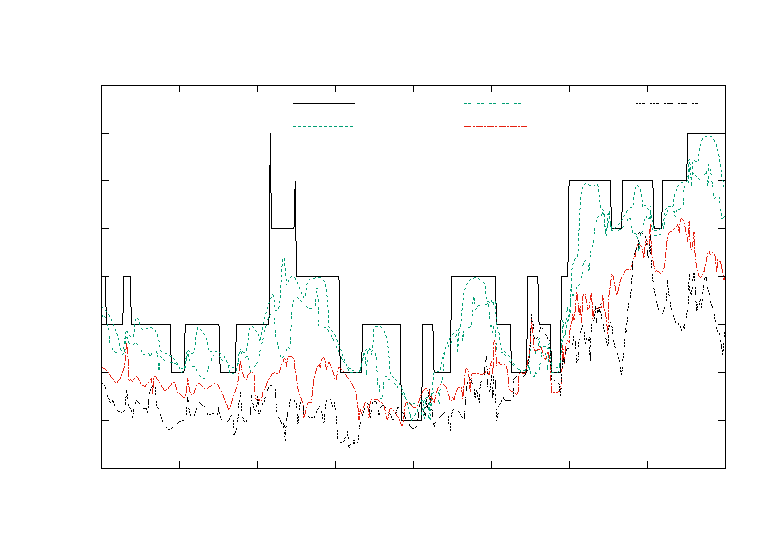
\includegraphics[width={360.00bp},height={252.00bp}]{zigzag-antiparallel-conductance-revise}}%
    \gplfronttext
  \end{picture}%
\endgroup
}
    \resizebox{0.45\textwidth}{!}{% GNUPLOT: LaTeX picture with Postscript
\begingroup
  % Encoding inside the plot.  In the header of your document, this encoding
  % should to defined, e.g., by using
  % \usepackage[cp1252,<other encodings>]{inputenc}
  % \inputencoding{cp1252}%
  \makeatletter
  \providecommand\color[2][]{%
    \GenericError{(gnuplot) \space\space\space\@spaces}{%
      Package color not loaded in conjunction with
      terminal option `colourtext'%
    }{See the gnuplot documentation for explanation.%
    }{Either use 'blacktext' in gnuplot or load the package
      color.sty in LaTeX.}%
    \renewcommand\color[2][]{}%
  }%
  \providecommand\includegraphics[2][]{%
    \GenericError{(gnuplot) \space\space\space\@spaces}{%
      Package graphicx or graphics not loaded%
    }{See the gnuplot documentation for explanation.%
    }{The gnuplot epslatex terminal needs graphicx.sty or graphics.sty.}%
    \renewcommand\includegraphics[2][]{}%
  }%
  \providecommand\rotatebox[2]{#2}%
  \@ifundefined{ifGPcolor}{%
    \newif\ifGPcolor
    \GPcolorfalse
  }{}%
  \@ifundefined{ifGPblacktext}{%
    \newif\ifGPblacktext
    \GPblacktexttrue
  }{}%
  % define a \g@addto@macro without @ in the name:
  \let\gplgaddtomacro\g@addto@macro
  % define empty templates for all commands taking text:
  \gdef\gplbacktext{}%
  \gdef\gplfronttext{}%
  \makeatother
  \ifGPblacktext
    % no textcolor at all
    \def\colorrgb#1{}%
    \def\colorgray#1{}%
  \else
    % gray or color?
    \ifGPcolor
      \def\colorrgb#1{\color[rgb]{#1}}%
      \def\colorgray#1{\color[gray]{#1}}%
      \expandafter\def\csname LTw\endcsname{\color{white}}%
      \expandafter\def\csname LTb\endcsname{\color{black}}%
      \expandafter\def\csname LTa\endcsname{\color{black}}%
      \expandafter\def\csname LT0\endcsname{\color[rgb]{1,0,0}}%
      \expandafter\def\csname LT1\endcsname{\color[rgb]{0,1,0}}%
      \expandafter\def\csname LT2\endcsname{\color[rgb]{0,0,1}}%
      \expandafter\def\csname LT3\endcsname{\color[rgb]{1,0,1}}%
      \expandafter\def\csname LT4\endcsname{\color[rgb]{0,1,1}}%
      \expandafter\def\csname LT5\endcsname{\color[rgb]{1,1,0}}%
      \expandafter\def\csname LT6\endcsname{\color[rgb]{0,0,0}}%
      \expandafter\def\csname LT7\endcsname{\color[rgb]{1,0.3,0}}%
      \expandafter\def\csname LT8\endcsname{\color[rgb]{0.5,0.5,0.5}}%
    \else
      % gray
      \def\colorrgb#1{\color{black}}%
      \def\colorgray#1{\color[gray]{#1}}%
      \expandafter\def\csname LTw\endcsname{\color{white}}%
      \expandafter\def\csname LTb\endcsname{\color{black}}%
      \expandafter\def\csname LTa\endcsname{\color{black}}%
      \expandafter\def\csname LT0\endcsname{\color{black}}%
      \expandafter\def\csname LT1\endcsname{\color{black}}%
      \expandafter\def\csname LT2\endcsname{\color{black}}%
      \expandafter\def\csname LT3\endcsname{\color{black}}%
      \expandafter\def\csname LT4\endcsname{\color{black}}%
      \expandafter\def\csname LT5\endcsname{\color{black}}%
      \expandafter\def\csname LT6\endcsname{\color{black}}%
      \expandafter\def\csname LT7\endcsname{\color{black}}%
      \expandafter\def\csname LT8\endcsname{\color{black}}%
    \fi
  \fi
    \setlength{\unitlength}{0.0500bp}%
    \ifx\gptboxheight\undefined%
      \newlength{\gptboxheight}%
      \newlength{\gptboxwidth}%
      \newsavebox{\gptboxtext}%
    \fi%
    \setlength{\fboxrule}{0.5pt}%
    \setlength{\fboxsep}{1pt}%
\begin{picture}(7200.00,5040.00)%
    \gplgaddtomacro\gplbacktext{%
      \csname LTb\endcsname%%
      \put(1000,4200){\makebox(0,0)[r]{\strut{}$D$}}%
      \put(682,704){\makebox(0,0)[r]{\strut{}$0$}}%
      \put(682,1112){\makebox(0,0)[r]{\strut{}$2$}}%
      \put(682,1521){\makebox(0,0)[r]{\strut{}$4$}}%
      \put(682,1929){\makebox(0,0)[r]{\strut{}$6$}}%
      \put(682,2337){\makebox(0,0)[r]{\strut{}$8$}}%
      \put(682,2746){\makebox(0,0)[r]{\strut{}$10$}}%
      \put(682,3154){\makebox(0,0)[r]{\strut{}$12$}}%
      \put(682,3562){\makebox(0,0)[r]{\strut{}$14$}}%
      \put(682,3971){\makebox(0,0)[r]{\strut{}$16$}}%
      \put(682,4379){\makebox(0,0)[r]{\strut{}$18$}}%
      \put(814,484){\makebox(0,0){\strut{}$-4$}}%
      \put(1563,484){\makebox(0,0){\strut{}$-3$}}%
      \put(2311,484){\makebox(0,0){\strut{}$-2$}}%
      \put(3060,484){\makebox(0,0){\strut{}$-1$}}%
      \put(3809,484){\makebox(0,0){\strut{}$0$}}%
      \put(4557,484){\makebox(0,0){\strut{}$1$}}%
      \put(5306,484){\makebox(0,0){\strut{}$2$}}%
      \put(6054,484){\makebox(0,0){\strut{}$3$}}%
      \put(6803,484){\makebox(0,0){\strut{}$4$}}%
    }%
    \gplgaddtomacro\gplfronttext{%
      \csname LTb\endcsname%%
      \put(209,2541){\rotatebox{-270}{\makebox(0,0){\strut{}$G(e^2/h)$}}}%
      \put(3808,154){\makebox(0,0){\strut{}$E(eV)$}}%
      \csname LTb\endcsname%%
      \put(2522,4206){\makebox(0,0)[r]{\strut{}$M=0$}}%
      \csname LTb\endcsname%%
      \put(2522,3986){\makebox(0,0)[r]{\strut{}$M=0.05$}}%
      \csname LTb\endcsname%%
      \put(4169,4206){\makebox(0,0)[r]{\strut{}$M=0.1$}}%
      \csname LTb\endcsname%%
      \put(4169,3986){\makebox(0,0)[r]{\strut{}$M=0.2$}}%
      \csname LTb\endcsname%%
      \put(5816,4206){\makebox(0,0)[r]{\strut{}$M=0.3$}}%
      \csname LTb\endcsname%%
      \put(3808,4709){\makebox(0,0){\strut{}Parallel}}%
    }%
    \gplbacktext
    \put(0,0){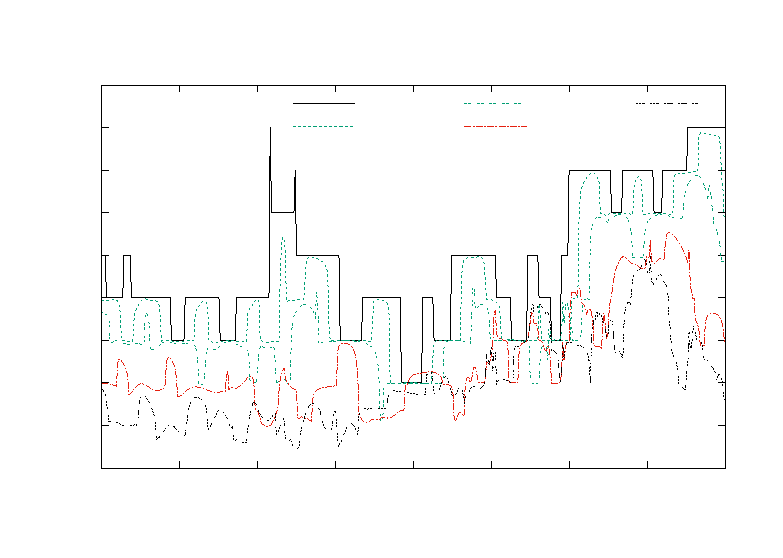
\includegraphics[width={360.00bp},height={252.00bp}]{zigzag-parallel-conductance-revise}}%
    \gplfronttext
  \end{picture}%
\endgroup
}
    \caption{A) Plot of borophene with armchair edge with 4 cells width for different magnetization of leads in AP configuration. B) Plot of borophene with armchair edge, and 4 unit cells width, for different magnetization of leads in P configuration. C) Plot of borophene with zigzag edge, with 4 unit cells width, for different magnetization of leads in P configuration. D) Plot of borophene with zigzag edge, and 4 unit cells width, for different magnetization of leads in AP configuration.}
    \label{fig:conductance}
\end{figure*}

Due to the possibility of using spin valves in electric, magnetic, and spin devices, two-dimensional (2D) materials have gained more and more attention in recent years\cite{gupta2015recent,an2019unveiling,mu2019electronic,an2020evaluating}. Numerous structural variables, such as flake size, thickness, edge shape, intrinsic defects, edge termination atoms, and others\cite{an2019unveiling,bekaroglu2010first,sun2008electronic,zhao2017spin}, can affect the characteristics of a material. The capability of transforming 2D-layered materials into nanoribbons has sparked research interest because these materials have the potential to become new electronic materials due to the unique magnetic properties in their electronic structure. The use of nanoribbons in spin electronics is a popular research topic.

Due to their exceptional spin-dependent properties, including ultra-long spin relaxation time and spin diffusion length, Rashba spin-orbit coupling (SOC), spin-valley locking, and quantum spin Hall Effect, 2D materials such as graphene\cite{novoselov2004electric}, black phosphorus (BP)\cite{liu2014phosphorene}, transition metal dichalcogenides (TMDCs)\cite{wang2012electronics}, and silicene\cite{guzman2007electronic} have created an excellent platform for spintronic research\cite{rahmani2019quantum,rahmani2020effect,davoodianidalik2018electronic,davoodianidalik2019structural}.

Brey and Fertig\cite{brey2007electronic} investigated the MR of an FM/graphene/FM junction in the limit of infinite width using the tight-binding concept. Since the conductance is only faintly affected by the relative magnetic orientations of the FM leads, they discovered that the MR is relatively low. A comparable device with two FM leads was examined by Ding et al.\cite{ding2009magnetic} using a continuous model.

The investigation of spin injection into graphene\cite{cho2007spin,ohishi2007giant}, magnetoresistance (MR)\cite{ding2009magnetic,wang2008quantum,chen2010edge,cheraghchi2012edge,yang2023magnetoresistance}, current-induced spin transfer torque (CISTT)\cite{zhou2010electronic}, and spin filtering impact in various graphene-based devices\cite{kang2011magnetic,sheng2010electronic,yang2013quantum}, etc., has also attracted a lot of attention in research. Spin-dependent transfer, such as STT, has been chiefly explored in two-dimensional materials like graphene, silicene, and silagraphene in earlier publications\cite{zhou2010magnetotransport,zhou2011spin,zhou2016spin,maher2022spin}.

Borophene, as a single layer of boron atoms, has gained interest recently because of its unique properties, including low density and high hardness, heat resistance (the melting point is significantly higher than silicene), and electrical conductance. Borophene has been efficiently synthesized on silver, copper, nickel, and gold substrates\cite{wu2019superconductivity,kiraly2013electronic,li2018surface}. Some of its exceptional properties, including novel magnetic\cite{pham2020electronic}, electrical, optical, thermodynamic\cite{meng2017investigation,lopez2016electronic,peng2016tuning}, mechanical\cite{mannix2015synthesis,wang2017first,giannopoulos2017first}, and superconducting\cite{penev2016convergence} properties, have already been studied.
\begin{figure*}[ht]
    \centering
    \resizebox{0.32\textwidth}{!}{% GNUPLOT: LaTeX picture with Postscript
\begin{latin}
\begingroup
  \makeatletter
  \providecommand\color[2][]{%
    \GenericError{(gnuplot) \space\space\space\@spaces}{%
      Package color not loaded in conjunction with
      terminal option `colourtext'%
    }{See the gnuplot documentation for explanation.%
    }{Either use 'blacktext' in gnuplot or load the package
      color.sty in LaTeX.}%
    \renewcommand\color[2][]{}%
  }%
  \providecommand\includegraphics[2][]{%
    \GenericError{(gnuplot) \space\space\space\@spaces}{%
      Package graphicx or graphics not loaded%
    }{See the gnuplot documentation for explanation.%
    }{The gnuplot epslatex terminal needs graphicx.sty or graphics.sty.}%
    \renewcommand\includegraphics[2][]{}%
  }%
  \providecommand\rotatebox[2]{#2}%
  \@ifundefined{ifGPcolor}{%
    \newif\ifGPcolor
    \GPcolorfalse
  }{}%
  \@ifundefined{ifGPblacktext}{%
    \newif\ifGPblacktext
    \GPblacktexttrue
  }{}%
  % define a \g@addto@macro without @ in the name:
  \let\gplgaddtomacro\g@addto@macro
  % define empty templates for all commands taking text:
  \gdef\gplbacktext{}%
  \gdef\gplfronttext{}%
  \makeatother
  \ifGPblacktext
    % no textcolor at all
    \def\colorrgb#1{}%
    \def\colorgray#1{}%
  \else
    % gray or color?
    \ifGPcolor
      \def\colorrgb#1{\color[rgb]{#1}}%
      \def\colorgray#1{\color[gray]{#1}}%
      \expandafter\def\csname LTw\endcsname{\color{white}}%
      \expandafter\def\csname LTb\endcsname{\color{black}}%
      \expandafter\def\csname LTa\endcsname{\color{black}}%
      \expandafter\def\csname LT0\endcsname{\color[rgb]{1,0,0}}%
      \expandafter\def\csname LT1\endcsname{\color[rgb]{0,1,0}}%
      \expandafter\def\csname LT2\endcsname{\color[rgb]{0,0,1}}%
      \expandafter\def\csname LT3\endcsname{\color[rgb]{1,0,1}}%
      \expandafter\def\csname LT4\endcsname{\color[rgb]{0,1,1}}%
      \expandafter\def\csname LT5\endcsname{\color[rgb]{1,1,0}}%
      \expandafter\def\csname LT6\endcsname{\color[rgb]{0,0,0}}%
      \expandafter\def\csname LT7\endcsname{\color[rgb]{1,0.3,0}}%
      \expandafter\def\csname LT8\endcsname{\color[rgb]{0.5,0.5,0.5}}%
    \else
      % gray
      \def\colorrgb#1{\color{black}}%
      \def\colorgray#1{\color[gray]{#1}}%
      \expandafter\def\csname LTw\endcsname{\color{white}}%
      \expandafter\def\csname LTb\endcsname{\color{black}}%
      \expandafter\def\csname LTa\endcsname{\color{black}}%
      \expandafter\def\csname LT0\endcsname{\color{black}}%
      \expandafter\def\csname LT1\endcsname{\color{black}}%
      \expandafter\def\csname LT2\endcsname{\color{black}}%
      \expandafter\def\csname LT3\endcsname{\color{black}}%
      \expandafter\def\csname LT4\endcsname{\color{black}}%
      \expandafter\def\csname LT5\endcsname{\color{black}}%
      \expandafter\def\csname LT6\endcsname{\color{black}}%
      \expandafter\def\csname LT7\endcsname{\color{black}}%
      \expandafter\def\csname LT8\endcsname{\color{black}}%
    \fi
  \fi
    \setlength{\unitlength}{0.0500bp}%
    \ifx\gptboxheight\undefined%
      \newlength{\gptboxheight}%
      \newlength{\gptboxwidth}%
      \newsavebox{\gptboxtext}%
    \fi%
    \setlength{\fboxrule}{0.5pt}%
    \setlength{\fboxsep}{1pt}%
\begin{picture}(3600.00,5040.00)%
    \gplgaddtomacro\gplbacktext{%
      \csname LTb\endcsname%%
      \put(1450,4200){\makebox(0,0)[r]{\strut{}$A$}}%
      \put(946,704){\makebox(0,0)[r]{\strut{}$-0.8$}}%
      \put(946,1439){\makebox(0,0)[r]{\strut{}$-0.7$}}%
      \put(946,2174){\makebox(0,0)[r]{\strut{}$-0.6$}}%
      \put(946,2909){\makebox(0,0)[r]{\strut{}$-0.5$}}%
      \put(946,3644){\makebox(0,0)[r]{\strut{}$-0.4$}}%
      \put(946,4379){\makebox(0,0)[r]{\strut{}$-0.3$}}%
      \put(1078,484){\makebox(0,0){\strut{}$0$}}%
      \put(1609,484){\makebox(0,0){\strut{}$0.5$}}%
      \put(2141,484){\makebox(0,0){\strut{}$1$}}%
      \put(2672,484){\makebox(0,0){\strut{}$1.5$}}%
      \put(3203,484){\makebox(0,0){\strut{}$2$}}%
      \put(1089,2909){\makebox(0,0)[l]{\strut{}$8\uparrow$}}%
      \put(1344,1439){\makebox(0,0)[l]{\strut{}$8\downarrow$}}%
      \put(1482,2909){\makebox(0,0)[l]{\strut{}$9\uparrow$}}%
      \put(1981,2174){\makebox(0,0)[l]{\strut{}$9\downarrow$}}%
    }%
    \gplgaddtomacro\gplfronttext{%
      \csname LTb\endcsname%%
      \put(209,2541){\rotatebox{-270}{\makebox(0,0){\strut{}$E(eV)$}}}%
      \put(2140,154){\makebox(0,0){\strut{}$k_x$}}%
      \csname LTb\endcsname%%
      \put(2140,4709){\makebox(0,0){\strut{}Left}}%
    }%
    \gplbacktext
    \put(0,0){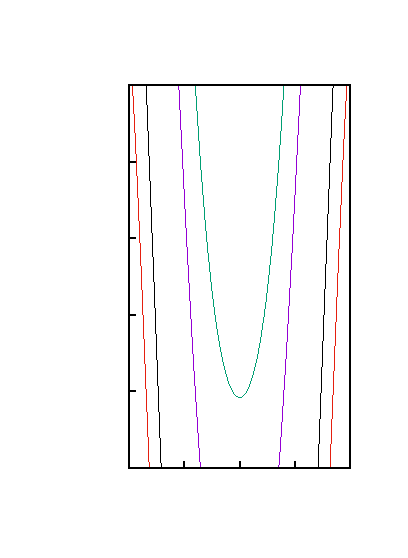
\includegraphics[width={180.00bp},height={252.00bp}]{Lborophene_band-revised}}%
    \gplfronttext
  \end{picture}%
\endgroup
\end{latin}}
    \resizebox{0.32\textwidth}{!}{% GNUPLOT: LaTeX picture with Postscript
\begin{latin}
\begingroup
  \makeatletter
  \providecommand\color[2][]{%
    \GenericError{(gnuplot) \space\space\space\@spaces}{%
      Package color not loaded in conjunction with
      terminal option `colourtext'%
    }{See the gnuplot documentation for explanation.%
    }{Either use 'blacktext' in gnuplot or load the package
      color.sty in LaTeX.}%
    \renewcommand\color[2][]{}%
  }%
  \providecommand\includegraphics[2][]{%
    \GenericError{(gnuplot) \space\space\space\@spaces}{%
      Package graphicx or graphics not loaded%
    }{See the gnuplot documentation for explanation.%
    }{The gnuplot epslatex terminal needs graphicx.sty or graphics.sty.}%
    \renewcommand\includegraphics[2][]{}%
  }%
  \providecommand\rotatebox[2]{#2}%
  \@ifundefined{ifGPcolor}{%
    \newif\ifGPcolor
    \GPcolorfalse
  }{}%
  \@ifundefined{ifGPblacktext}{%
    \newif\ifGPblacktext
    \GPblacktexttrue
  }{}%
  % define a \g@addto@macro without @ in the name:
  \let\gplgaddtomacro\g@addto@macro
  % define empty templates for all commands taking text:
  \gdef\gplbacktext{}%
  \gdef\gplfronttext{}%
  \makeatother
  \ifGPblacktext
    % no textcolor at all
    \def\colorrgb#1{}%
    \def\colorgray#1{}%
  \else
    % gray or color?
    \ifGPcolor
      \def\colorrgb#1{\color[rgb]{#1}}%
      \def\colorgray#1{\color[gray]{#1}}%
      \expandafter\def\csname LTw\endcsname{\color{white}}%
      \expandafter\def\csname LTb\endcsname{\color{black}}%
      \expandafter\def\csname LTa\endcsname{\color{black}}%
      \expandafter\def\csname LT0\endcsname{\color[rgb]{1,0,0}}%
      \expandafter\def\csname LT1\endcsname{\color[rgb]{0,1,0}}%
      \expandafter\def\csname LT2\endcsname{\color[rgb]{0,0,1}}%
      \expandafter\def\csname LT3\endcsname{\color[rgb]{1,0,1}}%
      \expandafter\def\csname LT4\endcsname{\color[rgb]{0,1,1}}%
      \expandafter\def\csname LT5\endcsname{\color[rgb]{1,1,0}}%
      \expandafter\def\csname LT6\endcsname{\color[rgb]{0,0,0}}%
      \expandafter\def\csname LT7\endcsname{\color[rgb]{1,0.3,0}}%
      \expandafter\def\csname LT8\endcsname{\color[rgb]{0.5,0.5,0.5}}%
    \else
      % gray
      \def\colorrgb#1{\color{black}}%
      \def\colorgray#1{\color[gray]{#1}}%
      \expandafter\def\csname LTw\endcsname{\color{white}}%
      \expandafter\def\csname LTb\endcsname{\color{black}}%
      \expandafter\def\csname LTa\endcsname{\color{black}}%
      \expandafter\def\csname LT0\endcsname{\color{black}}%
      \expandafter\def\csname LT1\endcsname{\color{black}}%
      \expandafter\def\csname LT2\endcsname{\color{black}}%
      \expandafter\def\csname LT3\endcsname{\color{black}}%
      \expandafter\def\csname LT4\endcsname{\color{black}}%
      \expandafter\def\csname LT5\endcsname{\color{black}}%
      \expandafter\def\csname LT6\endcsname{\color{black}}%
      \expandafter\def\csname LT7\endcsname{\color{black}}%
      \expandafter\def\csname LT8\endcsname{\color{black}}%
    \fi
  \fi
    \setlength{\unitlength}{0.0500bp}%
    \ifx\gptboxheight\undefined%
      \newlength{\gptboxheight}%
      \newlength{\gptboxwidth}%
      \newsavebox{\gptboxtext}%
    \fi%
    \setlength{\fboxrule}{0.5pt}%
    \setlength{\fboxsep}{1pt}%
\begin{picture}(3600.00,5040.00)%
    \gplgaddtomacro\gplbacktext{%
      \csname LTb\endcsname%%
      \put(1400,4200){\makebox(0,0)[r]{\strut{}$B$}}%
      \put(946,704){\makebox(0,0)[r]{\strut{}$-0.8$}}%
      \put(946,1439){\makebox(0,0)[r]{\strut{}$-0.7$}}%
      \put(946,2174){\makebox(0,0)[r]{\strut{}$-0.6$}}%
      \put(946,2909){\makebox(0,0)[r]{\strut{}$-0.5$}}%
      \put(946,3644){\makebox(0,0)[r]{\strut{}$-0.4$}}%
      \put(946,4379){\makebox(0,0)[r]{\strut{}$-0.3$}}%
      \put(1078,484){\makebox(0,0){\strut{}$0$}}%
      \put(1609,484){\makebox(0,0){\strut{}$0.5$}}%
      \put(2141,484){\makebox(0,0){\strut{}$1$}}%
      \put(2672,484){\makebox(0,0){\strut{}$1.5$}}%
      \put(3203,484){\makebox(0,0){\strut{}$2$}}%
      \put(1089,2909){\makebox(0,0)[l]{\strut{}$8\uparrow$}}%
      \put(1344,1439){\makebox(0,0)[l]{\strut{}$8\downarrow$}}%
      \put(1482,2909){\makebox(0,0)[l]{\strut{}$9\uparrow$}}%
      \put(1981,2174){\makebox(0,0)[l]{\strut{}$9\downarrow$}}%
    }%
    \gplgaddtomacro\gplfronttext{%
      \csname LTb\endcsname%%
      \put(209,2541){\rotatebox{-270}{\makebox(0,0){\strut{}$E(eV)$}}}%
      \put(2140,154){\makebox(0,0){\strut{}$k_x$}}%
      \csname LTb\endcsname%%
      \put(2140,4709){\makebox(0,0){\strut{}Center}}%
    }%
    \gplbacktext
    \put(0,0){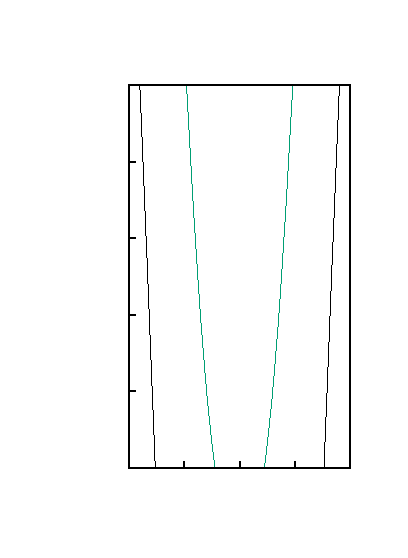
\includegraphics[width={180.00bp},height={252.00bp}]{Cborophene_band-revised}}%
    \gplfronttext
  \end{picture}%
\endgroup
\end{latin}}
    \resizebox{0.32\textwidth}{!}{% GNUPLOT: LaTeX picture with Postscript
\begingroup
  \makeatletter
  \providecommand\color[2][]{%
    \GenericError{(gnuplot) \space\space\space\@spaces}{%
      Package color not loaded in conjunction with
      terminal option `colourtext'%
    }{See the gnuplot documentation for explanation.%
    }{Either use 'blacktext' in gnuplot or load the package
      color.sty in LaTeX.}%
    \renewcommand\color[2][]{}%
  }%
  \providecommand\includegraphics[2][]{%
    \GenericError{(gnuplot) \space\space\space\@spaces}{%
      Package graphicx or graphics not loaded%
    }{See the gnuplot documentation for explanation.%
    }{The gnuplot epslatex terminal needs graphicx.sty or graphics.sty.}%
    \renewcommand\includegraphics[2][]{}%
  }%
  \providecommand\rotatebox[2]{#2}%
  \@ifundefined{ifGPcolor}{%
    \newif\ifGPcolor
    \GPcolorfalse
  }{}%
  \@ifundefined{ifGPblacktext}{%
    \newif\ifGPblacktext
    \GPblacktexttrue
  }{}%
  % define a \g@addto@macro without @ in the name:
  \let\gplgaddtomacro\g@addto@macro
  % define empty templates for all commands taking text:
  \gdef\gplbacktext{}%
  \gdef\gplfronttext{}%
  \makeatother
  \ifGPblacktext
    % no textcolor at all
    \def\colorrgb#1{}%
    \def\colorgray#1{}%
  \else
    % gray or color?
    \ifGPcolor
      \def\colorrgb#1{\color[rgb]{#1}}%
      \def\colorgray#1{\color[gray]{#1}}%
      \expandafter\def\csname LTw\endcsname{\color{white}}%
      \expandafter\def\csname LTb\endcsname{\color{black}}%
      \expandafter\def\csname LTa\endcsname{\color{black}}%
      \expandafter\def\csname LT0\endcsname{\color[rgb]{1,0,0}}%
      \expandafter\def\csname LT1\endcsname{\color[rgb]{0,1,0}}%
      \expandafter\def\csname LT2\endcsname{\color[rgb]{0,0,1}}%
      \expandafter\def\csname LT3\endcsname{\color[rgb]{1,0,1}}%
      \expandafter\def\csname LT4\endcsname{\color[rgb]{0,1,1}}%
      \expandafter\def\csname LT5\endcsname{\color[rgb]{1,1,0}}%
      \expandafter\def\csname LT6\endcsname{\color[rgb]{0,0,0}}%
      \expandafter\def\csname LT7\endcsname{\color[rgb]{1,0.3,0}}%
      \expandafter\def\csname LT8\endcsname{\color[rgb]{0.5,0.5,0.5}}%
    \else
      % gray
      \def\colorrgb#1{\color{black}}%
      \def\colorgray#1{\color[gray]{#1}}%
      \expandafter\def\csname LTw\endcsname{\color{white}}%
      \expandafter\def\csname LTb\endcsname{\color{black}}%
      \expandafter\def\csname LTa\endcsname{\color{black}}%
      \expandafter\def\csname LT0\endcsname{\color{black}}%
      \expandafter\def\csname LT1\endcsname{\color{black}}%
      \expandafter\def\csname LT2\endcsname{\color{black}}%
      \expandafter\def\csname LT3\endcsname{\color{black}}%
      \expandafter\def\csname LT4\endcsname{\color{black}}%
      \expandafter\def\csname LT5\endcsname{\color{black}}%
      \expandafter\def\csname LT6\endcsname{\color{black}}%
      \expandafter\def\csname LT7\endcsname{\color{black}}%
      \expandafter\def\csname LT8\endcsname{\color{black}}%
    \fi
  \fi
    \setlength{\unitlength}{0.0500bp}%
    \ifx\gptboxheight\undefined%
      \newlength{\gptboxheight}%
      \newlength{\gptboxwidth}%
      \newsavebox{\gptboxtext}%
    \fi%
    \setlength{\fboxrule}{0.5pt}%
    \setlength{\fboxsep}{1pt}%
\begin{picture}(3600.00,5040.00)%
    \gplgaddtomacro\gplbacktext{%
      \csname LTb\endcsname%%
      \put(1450,4200){\makebox(0,0)[r]{\strut{}$C$}}%
      \put(946,704){\makebox(0,0)[r]{\strut{}$-0.8$}}%
      \put(946,1439){\makebox(0,0)[r]{\strut{}$-0.7$}}%
      \put(946,2174){\makebox(0,0)[r]{\strut{}$-0.6$}}%
      \put(946,2909){\makebox(0,0)[r]{\strut{}$-0.5$}}%
      \put(946,3644){\makebox(0,0)[r]{\strut{}$-0.4$}}%
      \put(946,4379){\makebox(0,0)[r]{\strut{}$-0.3$}}%
      \put(1078,484){\makebox(0,0){\strut{}$0$}}%
      \put(1609,484){\makebox(0,0){\strut{}$0.5$}}%
      \put(2141,484){\makebox(0,0){\strut{}$1$}}%
      \put(2672,484){\makebox(0,0){\strut{}$1.5$}}%
      \put(3203,484){\makebox(0,0){\strut{}$2$}}%
      \put(1089,2909){\makebox(0,0)[l]{\strut{}$8\uparrow$}}%
      \put(1344,1439){\makebox(0,0)[l]{\strut{}$8\downarrow$}}%
      \put(1482,2909){\makebox(0,0)[l]{\strut{}$9\uparrow$}}%
      \put(1981,2174){\makebox(0,0)[l]{\strut{}$9\downarrow$}}%
    }%
    \gplgaddtomacro\gplfronttext{%
      \csname LTb\endcsname%%
      \put(209,2541){\rotatebox{-270}{\makebox(0,0){\strut{}$E(eV)$}}}%
      \put(2140,154){\makebox(0,0){\strut{}$k_x$}}%
      \csname LTb\endcsname%%
      \put(2140,4709){\makebox(0,0){\strut{}Right}}%
    }%
    \gplbacktext
    \put(0,0){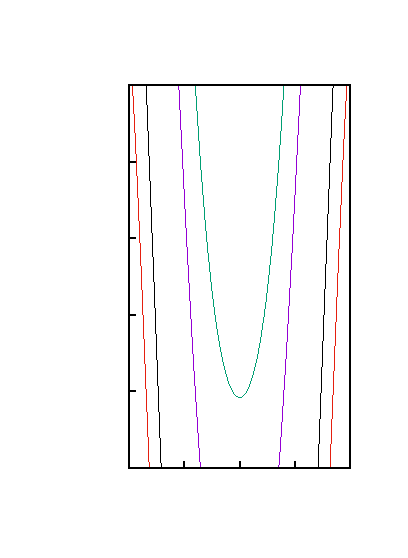
\includegraphics[width={180.00bp},height={252.00bp}]{Rborophene_band-revised}}%
    \gplfronttext
  \end{picture}%
\endgroup
}
    \resizebox{0.45\textwidth}{!}{% GNUPLOT: LaTeX picture with Postscript
\begin{latin}
\begingroup
  % Encoding inside the plot.  In the header of your document, this encoding
  % should to defined, e.g., by using
  % \usepackage[cp1252,<other encodings>]{inputenc}
  % \inputencoding{cp1252}%
  \makeatletter
  \providecommand\color[2][]{%
    \GenericError{(gnuplot) \space\space\space\@spaces}{%
      Package color not loaded in conjunction with
      terminal option `colourtext'%
    }{See the gnuplot documentation for explanation.%
    }{Either use 'blacktext' in gnuplot or load the package
      color.sty in LaTeX.}%
    \renewcommand\color[2][]{}%
  }%
  \providecommand\includegraphics[2][]{%
    \GenericError{(gnuplot) \space\space\space\@spaces}{%
      Package graphicx or graphics not loaded%
    }{See the gnuplot documentation for explanation.%
    }{The gnuplot epslatex terminal needs graphicx.sty or graphics.sty.}%
    \renewcommand\includegraphics[2][]{}%
  }%
  \providecommand\rotatebox[2]{#2}%
  \@ifundefined{ifGPcolor}{%
    \newif\ifGPcolor
    \GPcolorfalse
  }{}%
  \@ifundefined{ifGPblacktext}{%
    \newif\ifGPblacktext
    \GPblacktexttrue
  }{}%
  % define a \g@addto@macro without @ in the name:
  \let\gplgaddtomacro\g@addto@macro
  % define empty templates for all commands taking text:
  \gdef\gplbacktext{}%
  \gdef\gplfronttext{}%
  \makeatother
  \ifGPblacktext
    % no textcolor at all
    \def\colorrgb#1{}%
    \def\colorgray#1{}%
  \else
    % gray or color?
    \ifGPcolor
      \def\colorrgb#1{\color[rgb]{#1}}%
      \def\colorgray#1{\color[gray]{#1}}%
      \expandafter\def\csname LTw\endcsname{\color{white}}%
      \expandafter\def\csname LTb\endcsname{\color{black}}%
      \expandafter\def\csname LTa\endcsname{\color{black}}%
      \expandafter\def\csname LT0\endcsname{\color[rgb]{1,0,0}}%
      \expandafter\def\csname LT1\endcsname{\color[rgb]{0,1,0}}%
      \expandafter\def\csname LT2\endcsname{\color[rgb]{0,0,1}}%
      \expandafter\def\csname LT3\endcsname{\color[rgb]{1,0,1}}%
      \expandafter\def\csname LT4\endcsname{\color[rgb]{0,1,1}}%
      \expandafter\def\csname LT5\endcsname{\color[rgb]{1,1,0}}%
      \expandafter\def\csname LT6\endcsname{\color[rgb]{0,0,0}}%
      \expandafter\def\csname LT7\endcsname{\color[rgb]{1,0.3,0}}%
      \expandafter\def\csname LT8\endcsname{\color[rgb]{0.5,0.5,0.5}}%
    \else
      % gray
      \def\colorrgb#1{\color{black}}%
      \def\colorgray#1{\color[gray]{#1}}%
      \expandafter\def\csname LTw\endcsname{\color{white}}%
      \expandafter\def\csname LTb\endcsname{\color{black}}%
      \expandafter\def\csname LTa\endcsname{\color{black}}%
      \expandafter\def\csname LT0\endcsname{\color{black}}%
      \expandafter\def\csname LT1\endcsname{\color{black}}%
      \expandafter\def\csname LT2\endcsname{\color{black}}%
      \expandafter\def\csname LT3\endcsname{\color{black}}%
      \expandafter\def\csname LT4\endcsname{\color{black}}%
      \expandafter\def\csname LT5\endcsname{\color{black}}%
      \expandafter\def\csname LT6\endcsname{\color{black}}%
      \expandafter\def\csname LT7\endcsname{\color{black}}%
      \expandafter\def\csname LT8\endcsname{\color{black}}%
    \fi
  \fi
    \setlength{\unitlength}{0.0500bp}%
    \ifx\gptboxheight\undefined%
      \newlength{\gptboxheight}%
      \newlength{\gptboxwidth}%
      \newsavebox{\gptboxtext}%
    \fi%
    \setlength{\fboxrule}{0.5pt}%
    \setlength{\fboxsep}{1pt}%
\begin{picture}(7200.00,5040.00)%
    \gplgaddtomacro\gplbacktext{%
      \csname LTb\endcsname%%
      \put(1200,4200){\makebox(0,0)[r]{\strut{}$D$}}%
      \put(814,704){\makebox(0,0)[r]{\strut{}$1$}}%
      \put(814,1229){\makebox(0,0)[r]{\strut{}$1.5$}}%
      \put(814,1754){\makebox(0,0)[r]{\strut{}$2$}}%
      \put(814,2279){\makebox(0,0)[r]{\strut{}$2.5$}}%
      \put(814,2804){\makebox(0,0)[r]{\strut{}$3$}}%
      \put(814,3329){\makebox(0,0)[r]{\strut{}$3.5$}}%
      \put(814,3854){\makebox(0,0)[r]{\strut{}$4$}}%
      \put(814,4379){\makebox(0,0)[r]{\strut{}$4.5$}}%
      \put(946,484){\makebox(0,0){\strut{}$-1$}}%
      \put(2117,484){\makebox(0,0){\strut{}$-0.8$}}%
      \put(3289,484){\makebox(0,0){\strut{}$-0.6$}}%
      \put(4460,484){\makebox(0,0){\strut{}$-0.4$}}%
      \put(5632,484){\makebox(0,0){\strut{}$-0.2$}}%
      \put(6803,484){\makebox(0,0){\strut{}$0$}}%
    }%
    \gplgaddtomacro\gplfronttext{%
      \csname LTb\endcsname%%
      \put(209,2541){\rotatebox{-270}{\makebox(0,0){\strut{}$G(e^2/h)$}}}%
      \put(3874,154){\makebox(0,0){\strut{}$E(eV)$}}%
      \csname LTb\endcsname%%
      \put(2522,4206){\makebox(0,0)[r]{\strut{}$M=0$}}%
      \csname LTb\endcsname%%
      \put(2522,3986){\makebox(0,0)[r]{\strut{}$M=0.05$}}%
      \csname LTb\endcsname%%
      \put(4169,4206){\makebox(0,0)[r]{\strut{}$M=0.1$}}%
      \csname LTb\endcsname%%
      \put(4169,3986){\makebox(0,0)[r]{\strut{}$M=0.2$}}%
      \csname LTb\endcsname%%
      \put(5816,4206){\makebox(0,0)[r]{\strut{}$M=0.3$}}%
      \csname LTb\endcsname%%
      \put(3874,4709){\makebox(0,0){\strut{}Parallel}}%
    }%
    \gplbacktext
    \put(0,0){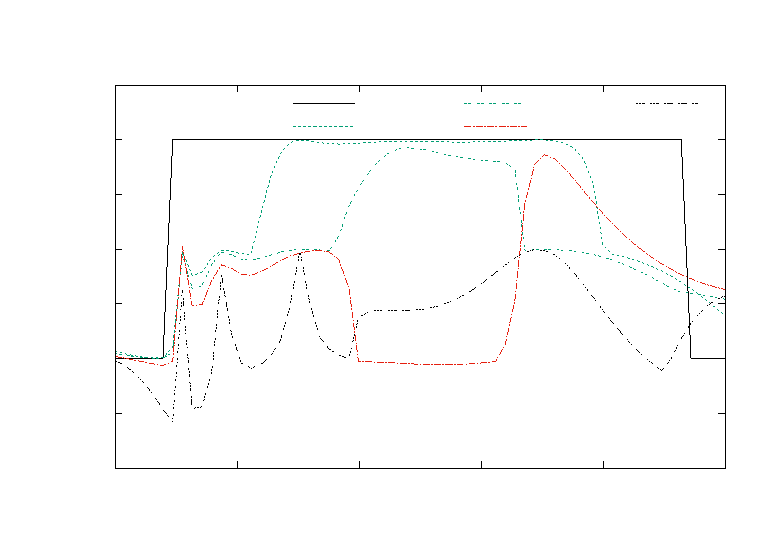
\includegraphics[width={360.00bp},height={252.00bp}]{armchair-parallel-conductance-1to0-revise}}%
    \gplfronttext
  \end{picture}%
\endgroup
\end{latin}}
    \resizebox{0.45\textwidth}{!}{\input{armchair-Antiparallel-conductance-1to0-revise.tex}}
    \caption{A, B, C) In the left lead, for an even number of atoms in the supercell, for example, the band number 8 (or 9) corresponds with atom number $8(9)$ is split into two subbands of spin up $(8^\uparrow)$ and spin down $(8\downarrow)$ when spin interaction is included: A) In the P configuration, the $(8\uparrow)$ subbands in both the left and right leads are placed above the $(8\downarrow)$ subbands with the same parity, and therefore electron transport is allowed. B) In AP configurations, the $(8\uparrow)$, in one lead, is located higher than the $(8\downarrow)$ subband on the same lead, while in the other lead, the $(8\uparrow)$ is located lower $(8\downarrow)$ subband with the opposite parity and, therefore electron transfer is not allowed. D, E) Plot of conductance in the same energy ranges of band structure for P and AP configurations.}
    \label{fig:bandconductance}
\end{figure*}

The atom of boron is the most comparable to that of carbon in the periodic table of elements. However, boron has a different topological class than carbon due to its lower spin-orbit coupling (SOC) and fewer valence electrons. In the case of graphene, silicene, and silographene, almost complete calculations for spin transport have been performed\cite{maher2022spin,chen2010electronic,qin2015origin,ding2014spin,zhou2015symmetry,schneider2014density}. In addition to conductance in P and AP configurations as well as arbitrary relative angles of magnetization of the leads have been investigated, calculations for MR and STT in the spin valve device with CPP structure have also been performed, and the results have been presented.

Various boron-based structures have been discovered, including clusters, fullerene cages, nanotubes, and 2D structures\cite{wu2012two,penev2012polymorphism,zhai2014observation,ciuparu2004synthesis}, which are classified as $\alpha$, $\beta$, $\chi$, $\psi$, $\delta$ nanostructures, which $\beta_{12}$, and $\chi\;3$ have been experimentally synthesized currently\cite{mannix2015synthesis,feng2016experimental}. The $\beta_{12}$-borophene, like graphene and silicene, has Dirac cones with $p_z$ as an important orbital, responsible for the unusual Electronic and transport properties of the material\cite{tang2007novel,ullah2020bat,jafari2020electronic}. Furthermore, in the development of the electronic industry, borophene establishes effective contact with many 2D semiconductors, lowering contact resistance and improving the performance of future 2D transistors\cite{yang2017interfacial}.
In $\beta_{12}$-borophene, only a few calculations have been done for the spin valve device with CIP structure, and the void of these various calculations, including P and AP conductance and MR and STT, is felt in the spin valve CPP structure for $\beta_{12}$-borophene\cite{yang2017interfacial}.

This paper examines the theoretical analysis of spin-dependent transport and spin-transport torque for a borophene-based FM/normal/FM junction. It is necessary to formulate spin-dependent tunneling currents in MTJ using a suitable framework to enhance the theoretical description of magnetoresistance. For this purpose, the Landauer formalism\cite{ezawa2017triplet}, based on the non-equilibrium Green's function (NEGF)\cite{slonczewski1989j}, is introduced as an acceptable and widely used approach.

Here, first, the conductance of borophene is calculated for both P and AP configurations, and zero conductances at some energies in the AP configuration and non-zero conductances in the P configuration are observed. This feature creates ON and OFF modes for use in switching. The spin-dependent combined scattering may explain the reason for zero conductance in the AP configuration, and the band selection filter can be represented using the parity of the subbands. In addition, on this basis, minor and frequent fluctuations in some energies are clarified. In the absence of disorder, a perfect MR plateau is found for the junction, which proves to be an excellent spin valve candidate.

The variations of spin transfer torque with Fermi energy and the relative angle between two electrode magnetizations are investigated at different ferromagnetic magnetic intensities. The calculations reveal that the STT per unit bias voltage ($e/4\pi$), as a function of the Fermi energy, reduces significantly near the Dirac point energy. Furthermore, a sinusoidal oscillating pattern can be recognized in the STT at unit bias voltage $V$ vs. the angle between the two electrode magnetizations, which intensifies as $M$ increases. Finally, in order to properly comprehend the system, $G$ is explored as a function of the relative angle between the two electrode magnetizations, as well as around the Dirac point energy.

The rest of the study is arranged as follows: In Section 2, we discuss the model and formulation based on which calculations are performed. Section 3 will present numerical findings for the spin-dependent conductance, MR, and STT for the zigzag and armchair edge instances, respectively. In Section 4, the paper concludes with a detailed discussion and a brief conclusion.

\section{Model and formulations:}
First-principles calculations and observations have proven that $\beta_{12}$-borophene is a stable two-dimensional sheet, like graphene\cite{feng2017dirac}. 

The $\beta_{12}$ structure is a rectangular lattice with P2MM symmetry, characterized by five atoms (a, b, c, d, and e) in Fig.\ref{fig:model}. The rectangular lattice constants are $2.92$ \AA\; and $5.06$ \AA\;\cite{zhang2016borophene}, respectively, implying that the boron-boron atom distance is $l = 1.69$ \AA.

\begin{figure*}
    \centering
    \resizebox{0.45\textwidth}{!}{% GNUPLOT: LaTeX picture with Postscript
\begingroup
  % Encoding inside the plot.  In the header of your document, this encoding
  % should to defined, e.g., by using
  % \usepackage[cp1252,<other encodings>]{inputenc}
  % \inputencoding{cp1252}%
  \makeatletter
  \providecommand\color[2][]{%
    \GenericError{(gnuplot) \space\space\space\@spaces}{%
      Package color not loaded in conjunction with
      terminal option `colourtext'%
    }{See the gnuplot documentation for explanation.%
    }{Either use 'blacktext' in gnuplot or load the package
      color.sty in LaTeX.}%
    \renewcommand\color[2][]{}%
  }%
  \providecommand\includegraphics[2][]{%
    \GenericError{(gnuplot) \space\space\space\@spaces}{%
      Package graphicx or graphics not loaded%
    }{See the gnuplot documentation for explanation.%
    }{The gnuplot epslatex terminal needs graphicx.sty or graphics.sty.}%
    \renewcommand\includegraphics[2][]{}%
  }%
  \providecommand\rotatebox[2]{#2}%
  \@ifundefined{ifGPcolor}{%
    \newif\ifGPcolor
    \GPcolorfalse
  }{}%
  \@ifundefined{ifGPblacktext}{%
    \newif\ifGPblacktext
    \GPblacktexttrue
  }{}%
  % define a \g@addto@macro without @ in the name:
  \let\gplgaddtomacro\g@addto@macro
  % define empty templates for all commands taking text:
  \gdef\gplbacktext{}%
  \gdef\gplfronttext{}%
  \makeatother
  \ifGPblacktext
    % no textcolor at all
    \def\colorrgb#1{}%
    \def\colorgray#1{}%
  \else
    % gray or color?
    \ifGPcolor
      \def\colorrgb#1{\color[rgb]{#1}}%
      \def\colorgray#1{\color[gray]{#1}}%
      \expandafter\def\csname LTw\endcsname{\color{white}}%
      \expandafter\def\csname LTb\endcsname{\color{black}}%
      \expandafter\def\csname LTa\endcsname{\color{black}}%
      \expandafter\def\csname LT0\endcsname{\color[rgb]{1,0,0}}%
      \expandafter\def\csname LT1\endcsname{\color[rgb]{0,1,0}}%
      \expandafter\def\csname LT2\endcsname{\color[rgb]{0,0,1}}%
      \expandafter\def\csname LT3\endcsname{\color[rgb]{1,0,1}}%
      \expandafter\def\csname LT4\endcsname{\color[rgb]{0,1,1}}%
      \expandafter\def\csname LT5\endcsname{\color[rgb]{1,1,0}}%
      \expandafter\def\csname LT6\endcsname{\color[rgb]{0,0,0}}%
      \expandafter\def\csname LT7\endcsname{\color[rgb]{1,0.3,0}}%
      \expandafter\def\csname LT8\endcsname{\color[rgb]{0.5,0.5,0.5}}%
    \else
      % gray
      \def\colorrgb#1{\color{black}}%
      \def\colorgray#1{\color[gray]{#1}}%
      \expandafter\def\csname LTw\endcsname{\color{white}}%
      \expandafter\def\csname LTb\endcsname{\color{black}}%
      \expandafter\def\csname LTa\endcsname{\color{black}}%
      \expandafter\def\csname LT0\endcsname{\color{black}}%
      \expandafter\def\csname LT1\endcsname{\color{black}}%
      \expandafter\def\csname LT2\endcsname{\color{black}}%
      \expandafter\def\csname LT3\endcsname{\color{black}}%
      \expandafter\def\csname LT4\endcsname{\color{black}}%
      \expandafter\def\csname LT5\endcsname{\color{black}}%
      \expandafter\def\csname LT6\endcsname{\color{black}}%
      \expandafter\def\csname LT7\endcsname{\color{black}}%
      \expandafter\def\csname LT8\endcsname{\color{black}}%
    \fi
  \fi
    \setlength{\unitlength}{0.0500bp}%
    \ifx\gptboxheight\undefined%
      \newlength{\gptboxheight}%
      \newlength{\gptboxwidth}%
      \newsavebox{\gptboxtext}%
    \fi%
    \setlength{\fboxrule}{0.5pt}%
    \setlength{\fboxsep}{1pt}%
\begin{picture}(7200.00,5040.00)%
    \gplgaddtomacro\gplbacktext{%
      \csname LTb\endcsname%%
      \put(1400,4600){\makebox(0,0)[r]{\strut{}$A$}}%
      \put(814,1077){\makebox(0,0)[r]{\strut{}$0$}}%
      \put(814,1635){\makebox(0,0)[r]{\strut{}$0.2$}}%
      \put(814,2193){\makebox(0,0)[r]{\strut{}$0.4$}}%
      \put(814,2751){\makebox(0,0)[r]{\strut{}$0.6$}}%
      \put(814,3309){\makebox(0,0)[r]{\strut{}$0.8$}}%
      \put(814,3867){\makebox(0,0)[r]{\strut{}$1$}}%
      \put(946,857){\makebox(0,0){\strut{}$-4$}}%
      \put(1678,857){\makebox(0,0){\strut{}$-3$}}%
      \put(2410,857){\makebox(0,0){\strut{}$-2$}}%
      \put(3142,857){\makebox(0,0){\strut{}$-1$}}%
      \put(3875,857){\makebox(0,0){\strut{}$0$}}%
      \put(4607,857){\makebox(0,0){\strut{}$1$}}%
      \put(5339,857){\makebox(0,0){\strut{}$2$}}%
      \put(6071,857){\makebox(0,0){\strut{}$3$}}%
      \put(6803,857){\makebox(0,0){\strut{}$4$}}%
    }%
    \gplgaddtomacro\gplfronttext{%
      \csname LTb\endcsname%%
      \put(209,2541){\rotatebox{-270}{\makebox(0,0){\strut{}MR}}}%
      \put(3874,527){\makebox(0,0){\strut{}$E(eV)$}}%
      \csname LTb\endcsname%%
      \put(2654,4867){\makebox(0,0)[r]{\strut{}$M=0$}}%
      \csname LTb\endcsname%%
      \put(2654,4647){\makebox(0,0)[r]{\strut{}$M=0.05$}}%
      \csname LTb\endcsname%%
      \put(4301,4867){\makebox(0,0)[r]{\strut{}$M=0.1$}}%
      \csname LTb\endcsname%%
      \put(4301,4647){\makebox(0,0)[r]{\strut{}$M=0.2$}}%
      \csname LTb\endcsname%%
      \put(5948,4867){\makebox(0,0)[r]{\strut{}$M=0.3$}}%
    }%
    \gplbacktext
    \put(0,0){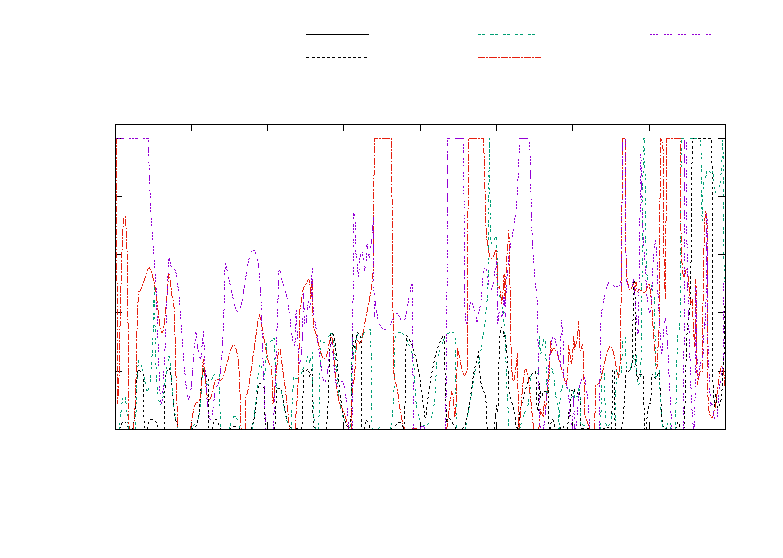
\includegraphics[width={360.00bp},height={252.00bp}]{MR-revise}}%
    \gplfronttext
  \end{picture}%
\endgroup
}
    \resizebox{0.45\textwidth}{!}{% GNUPLOT: LaTeX picture with Postscript
\begingroup
  % Encoding inside the plot.  In the header of your document, this encoding
  % should to defined, e.g., by using
  % \usepackage[cp1252,<other encodings>]{inputenc}
  % \inputencoding{cp1252}%s
  \makeatletter
  \providecommand\color[2][]{%
    \GenericError{(gnuplot) \space\space\space\@spaces}{%
      Package color not loaded in conjunction with
      terminal option `colourtext'%
    }{See the gnuplot documentation for explanation.%
    }{Either use 'blacktext' in gnuplot or load the package
      color.sty in LaTeX.}%
    \renewcommand\color[2][]{}%
  }%
  \providecommand\includegraphics[2][]{%
    \GenericError{(gnuplot) \space\space\space\@spaces}{%
      Package graphicx or graphics not loaded%
    }{See the gnuplot documentation for explanation.%
    }{The gnuplot epslatex terminal needs graphicx.sty or graphics.sty.}%
    \renewcommand\includegraphics[2][]{}%
  }%
  \providecommand\rotatebox[2]{#2}%
  \@ifundefined{ifGPcolor}{%
    \newif\ifGPcolor
    \GPcolorfalse
  }{}%
  \@ifundefined{ifGPblacktext}{%
    \newif\ifGPblacktext
    \GPblacktexttrue
  }{}%
  % define a \g@addto@macro without @ in the name:
  \let\gplgaddtomacro\g@addto@macro
  % define empty templates for all commands taking text:
  \gdef\gplbacktext{}%
  \gdef\gplfronttext{}%
  \makeatother
  \ifGPblacktext
    % no textcolor at all
    \def\colorrgb#1{}%
    \def\colorgray#1{}%
  \else
    % gray or color?
    \ifGPcolor
      \def\colorrgb#1{\color[rgb]{#1}}%
      \def\colorgray#1{\color[gray]{#1}}%
      \expandafter\def\csname LTw\endcsname{\color{white}}%
      \expandafter\def\csname LTb\endcsname{\color{black}}%
      \expandafter\def\csname LTa\endcsname{\color{black}}%
      \expandafter\def\csname LT0\endcsname{\color[rgb]{1,0,0}}%
      \expandafter\def\csname LT1\endcsname{\color[rgb]{0,1,0}}%
      \expandafter\def\csname LT2\endcsname{\color[rgb]{0,0,1}}%
      \expandafter\def\csname LT3\endcsname{\color[rgb]{1,0,1}}%
      \expandafter\def\csname LT4\endcsname{\color[rgb]{0,1,1}}%
      \expandafter\def\csname LT5\endcsname{\color[rgb]{1,1,0}}%
      \expandafter\def\csname LT6\endcsname{\color[rgb]{0,0,0}}%
      \expandafter\def\csname LT7\endcsname{\color[rgb]{1,0.3,0}}%
      \expandafter\def\csname LT8\endcsname{\color[rgb]{0.5,0.5,0.5}}%
    \else
      % gray
      \def\colorrgb#1{\color{black}}%
      \def\colorgray#1{\color[gray]{#1}}%
      \expandafter\def\csname LTw\endcsname{\color{white}}%
      \expandafter\def\csname LTb\endcsname{\color{black}}%
      \expandafter\def\csname LTa\endcsname{\color{black}}%
      \expandafter\def\csname LT0\endcsname{\color{black}}%
      \expandafter\def\csname LT1\endcsname{\color{black}}%
      \expandafter\def\csname LT2\endcsname{\color{black}}%
      \expandafter\def\csname LT3\endcsname{\color{black}}%
      \expandafter\def\csname LT4\endcsname{\color{black}}%
      \expandafter\def\csname LT5\endcsname{\color{black}}%
      \expandafter\def\csname LT6\endcsname{\color{black}}%
      \expandafter\def\csname LT7\endcsname{\color{black}}%
      \expandafter\def\csname LT8\endcsname{\color{black}}%
    \fi
  \fi
    \setlength{\unitlength}{0.0500bp}%
    \ifx\gptboxheight\undefined%
      \newlength{\gptboxheight}%
      \newlength{\gptboxwidth}%
      \newsavebox{\gptboxtext}%
    \fi%
    \setlength{\fboxrule}{0.5pt}%
    \setlength{\fboxsep}{1pt}%
\begin{picture}(7200.00,5040.00)%
    \gplgaddtomacro\gplbacktext{%
      \csname LTb\endcsname%%
      \put(1400,4600){\makebox(0,0)[r]{\strut{}$B$}}%
      \put(814,1077){\makebox(0,0)[r]{\strut{}$0$}}%
      \put(814,1635){\makebox(0,0)[r]{\strut{}$0.2$}}%
      \put(814,2193){\makebox(0,0)[r]{\strut{}$0.4$}}%
      \put(814,2751){\makebox(0,0)[r]{\strut{}$0.6$}}%
      \put(814,3309){\makebox(0,0)[r]{\strut{}$0.8$}}%
      \put(814,3867){\makebox(0,0)[r]{\strut{}$1$}}%
      \put(946,857){\makebox(0,0){\strut{}$-4$}}%
      \put(1678,857){\makebox(0,0){\strut{}$-3$}}%
      \put(2410,857){\makebox(0,0){\strut{}$-2$}}%
      \put(3142,857){\makebox(0,0){\strut{}$-1$}}%
      \put(3875,857){\makebox(0,0){\strut{}$0$}}%
      \put(4607,857){\makebox(0,0){\strut{}$1$}}%
      \put(5339,857){\makebox(0,0){\strut{}$2$}}%
      \put(6071,857){\makebox(0,0){\strut{}$3$}}%
      \put(6803,857){\makebox(0,0){\strut{}$4$}}%
    }%
    \gplgaddtomacro\gplfronttext{%
      \csname LTb\endcsname%%
      \put(209,2541){\rotatebox{-270}{\makebox(0,0){\strut{}MR}}}%
      \put(3874,527){\makebox(0,0){\strut{}$E(eV)$}}%
      \csname LTb\endcsname%%
      \put(2654,4867){\makebox(0,0)[r]{\strut{}$M=0$}}%
      \csname LTb\endcsname%%
      \put(2654,4647){\makebox(0,0)[r]{\strut{}$M=0.05$}}%
      \csname LTb\endcsname%%
      \put(4301,4867){\makebox(0,0)[r]{\strut{}$M=0.1$}}%
      \csname LTb\endcsname%%
      \put(4301,4647){\makebox(0,0)[r]{\strut{}$M=0.2$}}%
      \csname LTb\endcsname%%
      \put(5948,4867){\makebox(0,0)[r]{\strut{}$M=0.3$}}%
    }%
    \gplbacktext
    \put(0,0){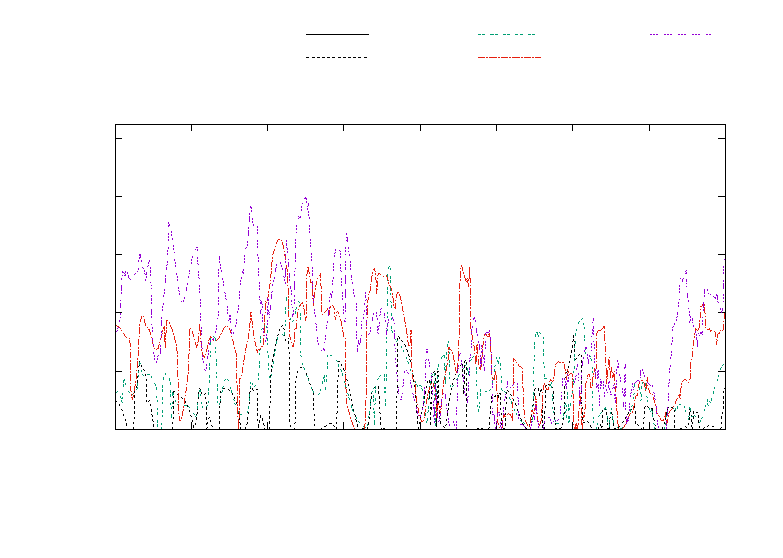
\includegraphics[width={360.00bp},height={252.00bp}]{MR_zig-revise}}%
    \gplfronttext
  \end{picture}%
\endgroup
}
     \caption{Mangnetoresistance(MR) of $\beta_{12}$-borophene in armchair and zigzag edges.}
    \label{fig:MR}
\end{figure*}

\begin{figure*}[ht]
    \centering
    \resizebox{0.45\textwidth}{!}{% GNUPLOT: LaTeX picture with Postscript
\begin{latin}
\begingroup
  % Encoding inside the plot.  In the header of your document, this encoding
  % should to defined, e.g., by using
  % \usepackage[cp1252,<other encodings>]{inputenc}
  % \inputencoding{cp1252}%
  \makeatletter
  \providecommand\color[2][]{%
    \GenericError{(gnuplot) \space\space\space\@spaces}{%
      Package color not loaded in conjunction with
      terminal option `colourtext'%
    }{See the gnuplot documentation for explanation.%
    }{Either use 'blacktext' in gnuplot or load the package
      color.sty in LaTeX.}%
    \renewcommand\color[2][]{}%
  }%
  \providecommand\includegraphics[2][]{%
    \GenericError{(gnuplot) \space\space\space\@spaces}{%
      Package graphicx or graphics not loaded%
    }{See the gnuplot documentation for explanation.%
    }{The gnuplot epslatex terminal needs graphicx.sty or graphics.sty.}%
    \renewcommand\includegraphics[2][]{}%
  }%
  \providecommand\rotatebox[2]{#2}%
  \@ifundefined{ifGPcolor}{%
    \newif\ifGPcolor
    \GPcolorfalse
  }{}%
  \@ifundefined{ifGPblacktext}{%
    \newif\ifGPblacktext
    \GPblacktexttrue
  }{}%
  % define a \g@addto@macro without @ in the name:
  \let\gplgaddtomacro\g@addto@macro
  % define empty templates for all commands taking text:
  \gdef\gplbacktext{}%
  \gdef\gplfronttext{}%
  \makeatother
  \ifGPblacktext
    % no textcolor at all
    \def\colorrgb#1{}%
    \def\colorgray#1{}%
  \else
    % gray or color?
    \ifGPcolor
      \def\colorrgb#1{\color[rgb]{#1}}%
      \def\colorgray#1{\color[gray]{#1}}%
      \expandafter\def\csname LTw\endcsname{\color{white}}%
      \expandafter\def\csname LTb\endcsname{\color{black}}%
      \expandafter\def\csname LTa\endcsname{\color{black}}%
      \expandafter\def\csname LT0\endcsname{\color[rgb]{1,0,0}}%
      \expandafter\def\csname LT1\endcsname{\color[rgb]{0,1,0}}%
      \expandafter\def\csname LT2\endcsname{\color[rgb]{0,0,1}}%
      \expandafter\def\csname LT3\endcsname{\color[rgb]{1,0,1}}%
      \expandafter\def\csname LT4\endcsname{\color[rgb]{0,1,1}}%
      \expandafter\def\csname LT5\endcsname{\color[rgb]{1,1,0}}%
      \expandafter\def\csname LT6\endcsname{\color[rgb]{0,0,0}}%
      \expandafter\def\csname LT7\endcsname{\color[rgb]{1,0.3,0}}%
      \expandafter\def\csname LT8\endcsname{\color[rgb]{0.5,0.5,0.5}}%
    \else
      % gray
      \def\colorrgb#1{\color{black}}%
      \def\colorgray#1{\color[gray]{#1}}%
      \expandafter\def\csname LTw\endcsname{\color{white}}%
      \expandafter\def\csname LTb\endcsname{\color{black}}%
      \expandafter\def\csname LTa\endcsname{\color{black}}%
      \expandafter\def\csname LT0\endcsname{\color{black}}%
      \expandafter\def\csname LT1\endcsname{\color{black}}%
      \expandafter\def\csname LT2\endcsname{\color{black}}%
      \expandafter\def\csname LT3\endcsname{\color{black}}%
      \expandafter\def\csname LT4\endcsname{\color{black}}%
      \expandafter\def\csname LT5\endcsname{\color{black}}%
      \expandafter\def\csname LT6\endcsname{\color{black}}%
      \expandafter\def\csname LT7\endcsname{\color{black}}%
      \expandafter\def\csname LT8\endcsname{\color{black}}%
    \fi
  \fi
    \setlength{\unitlength}{0.0500bp}%
    \ifx\gptboxheight\undefined%
      \newlength{\gptboxheight}%
      \newlength{\gptboxwidth}%
      \newsavebox{\gptboxtext}%
    \fi%
    \setlength{\fboxrule}{0.5pt}%
    \setlength{\fboxsep}{1pt}%
\begin{picture}(7200.00,5040.00)%
    \gplgaddtomacro\gplbacktext{%
      \csname LTb\endcsname%%
      \put(1300,4200){\makebox(0,0)[r]{\strut{}$A$}}%
      \put(946,704){\makebox(0,0)[r]{\strut{}$-0.3$}}%
      \put(946,1323){\makebox(0,0)[r]{\strut{}$-0.2$}}%
      \put(946,1942){\makebox(0,0)[r]{\strut{}$-0.1$}}%
      \put(946,2562){\makebox(0,0)[r]{\strut{}$0$}}%
      \put(946,3181){\makebox(0,0)[r]{\strut{}$0.1$}}%
      \put(946,3800){\makebox(0,0)[r]{\strut{}$0.2$}}%
      \put(946,4419){\makebox(0,0)[r]{\strut{}$0.3$}}%
      \put(1078,484){\makebox(0,0){\strut{}$0$}}%
      \put(2509,484){\makebox(0,0){\strut{}$0.5$}}%
      \put(3941,484){\makebox(0,0){\strut{}$1$}}%
      \put(5372,484){\makebox(0,0){\strut{}$1.5$}}%
      \put(6803,484){\makebox(0,0){\strut{}$2$}}%
    }%
    \gplgaddtomacro\gplfronttext{%
      \csname LTb\endcsname%%
      \put(209,2561){\rotatebox{-270}{\makebox(0,0){\strut{}$\tau/V$}}}%
      \put(3940,154){\makebox(0,0){\strut{}$\theta$}}%
      \csname LTb\endcsname%%
      \put(5816,4246){\makebox(0,0)[r]{\strut{}$M=0.05$}}%
      \csname LTb\endcsname%%
      \put(5816,4026){\makebox(0,0)[r]{\strut{}$M=0.10$}}%
      \csname LTb\endcsname%%
      \put(5816,3806){\makebox(0,0)[r]{\strut{}$M=0.20$}}%
      \csname LTb\endcsname%%
      \put(5816,3586){\makebox(0,0)[r]{\strut{}$M=0.30$}}%
      \csname LTb\endcsname%%
      \put(3940,4709){\makebox(0,0){\strut{}Spin Torque 2D}}%
    }%
    \gplbacktext
    \put(0,0){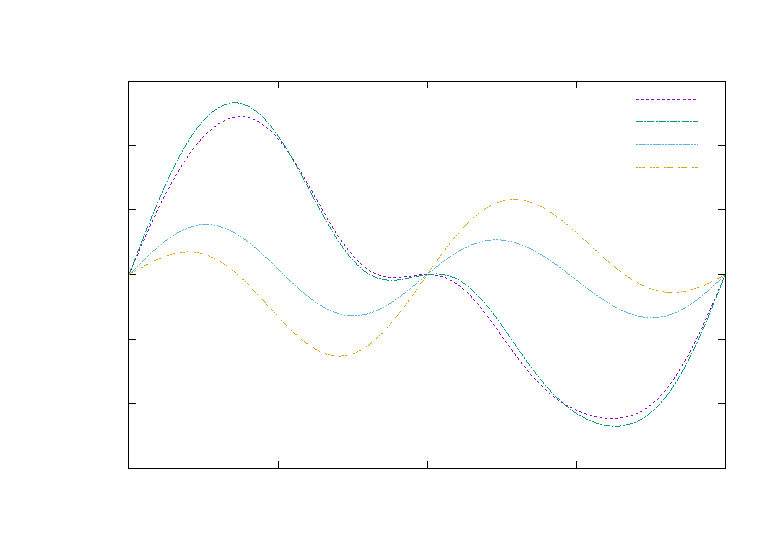
\includegraphics[width={360.00bp},height={252.00bp}]{stt}}%
    \gplfronttext
  \end{picture}%
\endgroup
\end{latin}}
    \resizebox{0.45\textwidth}{!}{% GNUPLOT: LaTeX picture with Postscript
\begingroup
  % Encoding inside the plot.  In the header of your document, this encoding
  % should to defined, e.g., by using
  % \usepackage[cp1252,<other encodings>]{inputenc}
  % \inputencoding{cp1252}%
  \makeatletter
  \providecommand\color[2][]{%
    \GenericError{(gnuplot) \space\space\space\@spaces}{%
      Package color not loaded in conjunction with
      terminal option `colourtext'%
    }{See the gnuplot documentation for explanation.%
    }{Either use 'blacktext' in gnuplot or load the package
      color.sty in LaTeX.}%
    \renewcommand\color[2][]{}%
  }%
  \providecommand\includegraphics[2][]{%
    \GenericError{(gnuplot) \space\space\space\@spaces}{%
      Package graphicx or graphics not loaded%
    }{See the gnuplot documentation for explanation.%
    }{The gnuplot epslatex terminal needs graphicx.sty or graphics.sty.}%
    \renewcommand\includegraphics[2][]{}%
  }%
  \providecommand\rotatebox[2]{#2}%
  \@ifundefined{ifGPcolor}{%
    \newif\ifGPcolor
    \GPcolorfalse
  }{}%
  \@ifundefined{ifGPblacktext}{%
    \newif\ifGPblacktext
    \GPblacktexttrue
  }{}%
  % define a \g@addto@macro without @ in the name:
  \let\gplgaddtomacro\g@addto@macro
  % define empty templates for all commands taking text:
  \gdef\gplbacktext{}%
  \gdef\gplfronttext{}%
  \makeatother
  \ifGPblacktext
    % no textcolor at all
    \def\colorrgb#1{}%
    \def\colorgray#1{}%
  \else
    % gray or color?
    \ifGPcolor
      \def\colorrgb#1{\color[rgb]{#1}}%
      \def\colorgray#1{\color[gray]{#1}}%
      \expandafter\def\csname LTw\endcsname{\color{white}}%
      \expandafter\def\csname LTb\endcsname{\color{black}}%
      \expandafter\def\csname LTa\endcsname{\color{black}}%
      \expandafter\def\csname LT0\endcsname{\color[rgb]{1,0,0}}%
      \expandafter\def\csname LT1\endcsname{\color[rgb]{0,1,0}}%
      \expandafter\def\csname LT2\endcsname{\color[rgb]{0,0,1}}%
      \expandafter\def\csname LT3\endcsname{\color[rgb]{1,0,1}}%
      \expandafter\def\csname LT4\endcsname{\color[rgb]{0,1,1}}%
      \expandafter\def\csname LT5\endcsname{\color[rgb]{1,1,0}}%
      \expandafter\def\csname LT6\endcsname{\color[rgb]{0,0,0}}%
      \expandafter\def\csname LT7\endcsname{\color[rgb]{1,0.3,0}}%
      \expandafter\def\csname LT8\endcsname{\color[rgb]{0.5,0.5,0.5}}%
    \else
      % gray
      \def\colorrgb#1{\color{black}}%
      \def\colorgray#1{\color[gray]{#1}}%
      \expandafter\def\csname LTw\endcsname{\color{white}}%
      \expandafter\def\csname LTb\endcsname{\color{black}}%
      \expandafter\def\csname LTa\endcsname{\color{black}}%
      \expandafter\def\csname LT0\endcsname{\color{black}}%
      \expandafter\def\csname LT1\endcsname{\color{black}}%
      \expandafter\def\csname LT2\endcsname{\color{black}}%
      \expandafter\def\csname LT3\endcsname{\color{black}}%
      \expandafter\def\csname LT4\endcsname{\color{black}}%
      \expandafter\def\csname LT5\endcsname{\color{black}}%
      \expandafter\def\csname LT6\endcsname{\color{black}}%
      \expandafter\def\csname LT7\endcsname{\color{black}}%
      \expandafter\def\csname LT8\endcsname{\color{black}}%
    \fi
  \fi
    \setlength{\unitlength}{0.0500bp}%
    \ifx\gptboxheight\undefined%
      \newlength{\gptboxheight}%
      \newlength{\gptboxwidth}%
      \newsavebox{\gptboxtext}%
    \fi%
    \setlength{\fboxrule}{0.5pt}%
    \setlength{\fboxsep}{1pt}%
\begin{picture}(7200.00,5040.00)%
    \gplgaddtomacro\gplbacktext{%
    }%
    \gplgaddtomacro\gplfronttext{%
      \csname LTb\endcsname%%
      \put(1300,3900){\makebox(0,0)[r]{\strut{}$B$}}%
      \put(936,674){\makebox(0,0){\strut{}$-4$}}%
      \put(1602,674){\makebox(0,0){\strut{}$-3$}}%
      \put(2268,674){\makebox(0,0){\strut{}$-2$}}%
      \put(2934,674){\makebox(0,0){\strut{}$-1$}}%
      \put(3600,674){\makebox(0,0){\strut{}$0$}}%
      \put(4266,674){\makebox(0,0){\strut{}$1$}}%
      \put(4932,674){\makebox(0,0){\strut{}$2$}}%
      \put(5598,674){\makebox(0,0){\strut{}$3$}}%
      \put(6264,674){\makebox(0,0){\strut{}$4$}}%
      \put(3600,344){\makebox(0,0){\strut{}$E(eV)$}}%
      \put(693,917){\makebox(0,0)[r]{\strut{}$-6$}}%
      \put(693,1318){\makebox(0,0)[r]{\strut{}$-4$}}%
      \put(693,1719){\makebox(0,0)[r]{\strut{}$-2$}}%
      \put(693,2120){\makebox(0,0)[r]{\strut{}$0$}}%
      \put(693,2520){\makebox(0,0)[r]{\strut{}$2$}}%
      \put(693,2920){\makebox(0,0)[r]{\strut{}$4$}}%
      \put(693,3321){\makebox(0,0)[r]{\strut{}$6$}}%
      \put(693,3722){\makebox(0,0)[r]{\strut{}$8$}}%
      \put(693,4123){\makebox(0,0)[r]{\strut{}$10$}}%
      \put(363,2520){\rotatebox{-270}{\makebox(0,0){\strut{}$\tau$}}}%
      \put(6795,917){\makebox(0,0)[l]{\strut{}$0$}}%
      \put(6795,1237){\makebox(0,0)[l]{\strut{}$0.2$}}%
      \put(6795,1558){\makebox(0,0)[l]{\strut{}$0.4$}}%
      \put(6795,1878){\makebox(0,0)[l]{\strut{}$0.6$}}%
      \put(6795,2199){\makebox(0,0)[l]{\strut{}$0.8$}}%
      \put(6795,2520){\makebox(0,0)[l]{\strut{}$1$}}%
      \put(6795,2840){\makebox(0,0)[l]{\strut{}$1.2$}}%
      \put(6795,3161){\makebox(0,0)[l]{\strut{}$1.4$}}%
      \put(6795,3481){\makebox(0,0)[l]{\strut{}$1.6$}}%
      \put(6795,3802){\makebox(0,0)[l]{\strut{}$1.8$}}%
      \put(6795,4123){\makebox(0,0)[l]{\strut{}$2$}}%
      \put(7257,2520){\rotatebox{-270}{\makebox(0,0){\strut{}$\theta$}}}%
      \put(3600,4453){\makebox(0,0){\strut{}$M=0.1$}}%
    }%
    \gplbacktext
    \put(0,0){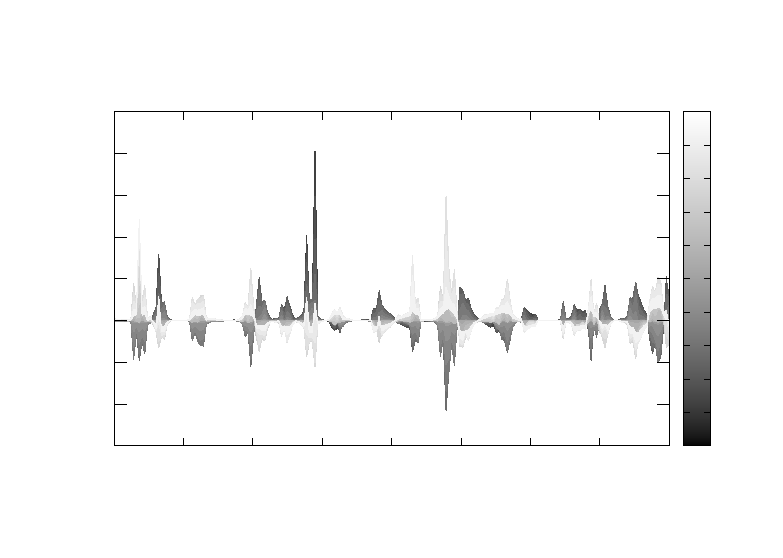
\includegraphics[width={360.00bp},height={252.00bp}]{stt-energy3d-0.1}}%
    \gplfronttext
  \end{picture}%
\endgroup
}
    \resizebox{0.45\textwidth}{!}{% GNUPLOT: LaTeX picture with Postscript
\begingroup
  % Encoding inside the plot.  In the header of your document, this encoding
  % should to defined, e.g., by using
  % \usepackage[cp1252,<other encodings>]{inputenc}
  % \inputencoding{cp1252}%
  \makeatletter
  \providecommand\color[2][]{%
    \GenericError{(gnuplot) \space\space\space\@spaces}{%
      Package color not loaded in conjunction with
      terminal option `colourtext'%
    }{See the gnuplot documentation for explanation.%
    }{Either use 'blacktext' in gnuplot or load the package
      color.sty in LaTeX.}%
    \renewcommand\color[2][]{}%
  }%
  \providecommand\includegraphics[2][]{%
    \GenericError{(gnuplot) \space\space\space\@spaces}{%
      Package graphicx or graphics not loaded%
    }{See the gnuplot documentation for explanation.%
    }{The gnuplot epslatex terminal needs graphicx.sty or graphics.sty.}%
    \renewcommand\includegraphics[2][]{}%
  }%
  \providecommand\rotatebox[2]{#2}%
  \@ifundefined{ifGPcolor}{%
    \newif\ifGPcolor
    \GPcolorfalse
  }{}%
  \@ifundefined{ifGPblacktext}{%
    \newif\ifGPblacktext
    \GPblacktexttrue
  }{}%
  % define a \g@addto@macro without @ in the name:
  \let\gplgaddtomacro\g@addto@macro
  % define empty templates for all commands taking text:
  \gdef\gplbacktext{}%
  \gdef\gplfronttext{}%
  \makeatother
  \ifGPblacktext
    % no textcolor at all
    \def\colorrgb#1{}%
    \def\colorgray#1{}%
  \else
    % gray or color?
    \ifGPcolor
      \def\colorrgb#1{\color[rgb]{#1}}%
      \def\colorgray#1{\color[gray]{#1}}%
      \expandafter\def\csname LTw\endcsname{\color{white}}%
      \expandafter\def\csname LTb\endcsname{\color{black}}%
      \expandafter\def\csname LTa\endcsname{\color{black}}%
      \expandafter\def\csname LT0\endcsname{\color[rgb]{1,0,0}}%
      \expandafter\def\csname LT1\endcsname{\color[rgb]{0,1,0}}%
      \expandafter\def\csname LT2\endcsname{\color[rgb]{0,0,1}}%
      \expandafter\def\csname LT3\endcsname{\color[rgb]{1,0,1}}%
      \expandafter\def\csname LT4\endcsname{\color[rgb]{0,1,1}}%
      \expandafter\def\csname LT5\endcsname{\color[rgb]{1,1,0}}%
      \expandafter\def\csname LT6\endcsname{\color[rgb]{0,0,0}}%
      \expandafter\def\csname LT7\endcsname{\color[rgb]{1,0.3,0}}%
      \expandafter\def\csname LT8\endcsname{\color[rgb]{0.5,0.5,0.5}}%
    \else
      % gray
      \def\colorrgb#1{\color{black}}%
      \def\colorgray#1{\color[gray]{#1}}%
      \expandafter\def\csname LTw\endcsname{\color{white}}%
      \expandafter\def\csname LTb\endcsname{\color{black}}%
      \expandafter\def\csname LTa\endcsname{\color{black}}%
      \expandafter\def\csname LT0\endcsname{\color{black}}%
      \expandafter\def\csname LT1\endcsname{\color{black}}%
      \expandafter\def\csname LT2\endcsname{\color{black}}%
      \expandafter\def\csname LT3\endcsname{\color{black}}%
      \expandafter\def\csname LT4\endcsname{\color{black}}%
      \expandafter\def\csname LT5\endcsname{\color{black}}%
      \expandafter\def\csname LT6\endcsname{\color{black}}%
      \expandafter\def\csname LT7\endcsname{\color{black}}%
      \expandafter\def\csname LT8\endcsname{\color{black}}%
    \fi
  \fi
    \setlength{\unitlength}{0.0500bp}%
    \ifx\gptboxheight\undefined%
      \newlength{\gptboxheight}%
      \newlength{\gptboxwidth}%
      \newsavebox{\gptboxtext}%
    \fi%
    \setlength{\fboxrule}{0.5pt}%
    \setlength{\fboxsep}{1pt}%
\begin{picture}(7200.00,5040.00)%
    \gplgaddtomacro\gplbacktext{%
    }%
    \gplgaddtomacro\gplfronttext{%
      \csname LTb\endcsname%%
      \put(1300,3900){\makebox(0,0)[r]{\strut{}$C$}}%
      \put(936,674){\makebox(0,0){\strut{}$-4$}}%
      \put(1602,674){\makebox(0,0){\strut{}$-3$}}%
      \put(2268,674){\makebox(0,0){\strut{}$-2$}}%
      \put(2934,674){\makebox(0,0){\strut{}$-1$}}%
      \put(3600,674){\makebox(0,0){\strut{}$0$}}%
      \put(4266,674){\makebox(0,0){\strut{}$1$}}%
      \put(4932,674){\makebox(0,0){\strut{}$2$}}%
      \put(5598,674){\makebox(0,0){\strut{}$3$}}%
      \put(6264,674){\makebox(0,0){\strut{}$4$}}%
      \put(3600,344){\makebox(0,0){\strut{}$E(eV)$}}%
      \put(693,917){\makebox(0,0)[r]{\strut{}$-4$}}%
      \put(693,1375){\makebox(0,0)[r]{\strut{}$-2$}}%
      \put(693,1833){\makebox(0,0)[r]{\strut{}$0$}}%
      \put(693,2291){\makebox(0,0)[r]{\strut{}$2$}}%
      \put(693,2749){\makebox(0,0)[r]{\strut{}$4$}}%
      \put(693,3207){\makebox(0,0)[r]{\strut{}$6$}}%
      \put(693,3665){\makebox(0,0)[r]{\strut{}$8$}}%
      \put(693,4123){\makebox(0,0)[r]{\strut{}$10$}}%
      \put(363,2520){\rotatebox{-270}{\makebox(0,0){\strut{}$\tau$}}}%
      \put(6795,917){\makebox(0,0)[l]{\strut{}$0$}}%
      \put(6795,1237){\makebox(0,0)[l]{\strut{}$0.2$}}%
      \put(6795,1558){\makebox(0,0)[l]{\strut{}$0.4$}}%
      \put(6795,1878){\makebox(0,0)[l]{\strut{}$0.6$}}%
      \put(6795,2199){\makebox(0,0)[l]{\strut{}$0.8$}}%
      \put(6795,2520){\makebox(0,0)[l]{\strut{}$1$}}%
      \put(6795,2840){\makebox(0,0)[l]{\strut{}$1.2$}}%
      \put(6795,3161){\makebox(0,0)[l]{\strut{}$1.4$}}%
      \put(6795,3481){\makebox(0,0)[l]{\strut{}$1.6$}}%
      \put(6795,3802){\makebox(0,0)[l]{\strut{}$1.8$}}%
      \put(6795,4123){\makebox(0,0)[l]{\strut{}$2$}}%
      \put(7257,2520){\rotatebox{-270}{\makebox(0,0){\strut{}$\theta$}}}%
      \put(3600,4453){\makebox(0,0){\strut{}$M=0.2$}}%
    }%
    \gplbacktext
    \put(0,0){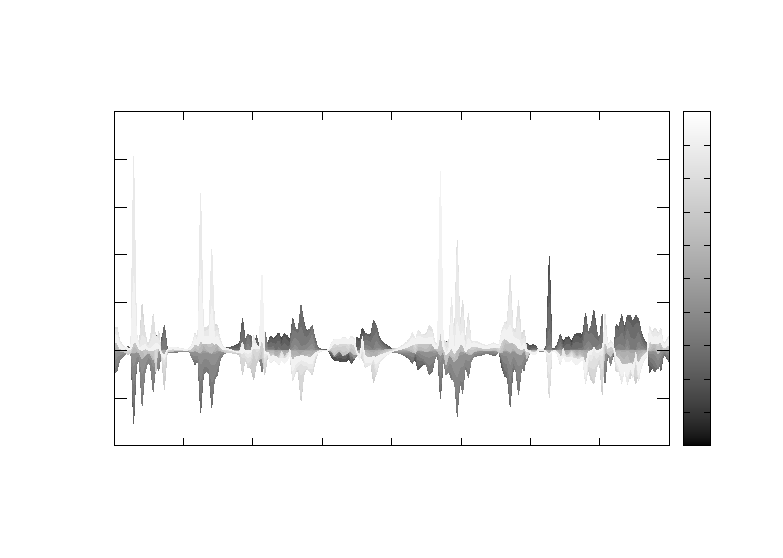
\includegraphics[width={360.00bp},height={252.00bp}]{stt-energy3d-0.2}}%
    \gplfronttext
  \end{picture}%
\endgroup
}
    \resizebox{0.45\textwidth}{!}{% GNUPLOT: LaTeX picture with Postscript
\begingroup
  % Encoding inside the plot.  In the header of your document, this encoding
  % should to defined, e.g., by using
  % \usepackage[cp1252,<other encodings>]{inputenc}
  % \inputencoding{cp1252}%
  \makeatletter
  \providecommand\color[2][]{%
    \GenericError{(gnuplot) \space\space\space\@spaces}{%
      Package color not loaded in conjunction with
      terminal option `colourtext'%
    }{See the gnuplot documentation for explanation.%
    }{Either use 'blacktext' in gnuplot or load the package
      color.sty in LaTeX.}%
    \renewcommand\color[2][]{}%
  }%
  \providecommand\includegraphics[2][]{%
    \GenericError{(gnuplot) \space\space\space\@spaces}{%
      Package graphicx or graphics not loaded%
    }{See the gnuplot documentation for explanation.%
    }{The gnuplot epslatex terminal needs graphicx.sty or graphics.sty.}%
    \renewcommand\includegraphics[2][]{}%
  }%
  \providecommand\rotatebox[2]{#2}%
  \@ifundefined{ifGPcolor}{%
    \newif\ifGPcolor
    \GPcolorfalse
  }{}%
  \@ifundefined{ifGPblacktext}{%
    \newif\ifGPblacktext
    \GPblacktexttrue
  }{}%
  % define a \g@addto@macro without @ in the name:
  \let\gplgaddtomacro\g@addto@macro
  % define empty templates for all commands taking text:
  \gdef\gplbacktext{}%
  \gdef\gplfronttext{}%
  \makeatother
  \ifGPblacktext
    % no textcolor at all
    \def\colorrgb#1{}%
    \def\colorgray#1{}%
  \else
    % gray or color?
    \ifGPcolor
      \def\colorrgb#1{\color[rgb]{#1}}%
      \def\colorgray#1{\color[gray]{#1}}%
      \expandafter\def\csname LTw\endcsname{\color{white}}%
      \expandafter\def\csname LTb\endcsname{\color{black}}%
      \expandafter\def\csname LTa\endcsname{\color{black}}%
      \expandafter\def\csname LT0\endcsname{\color[rgb]{1,0,0}}%
      \expandafter\def\csname LT1\endcsname{\color[rgb]{0,1,0}}%
      \expandafter\def\csname LT2\endcsname{\color[rgb]{0,0,1}}%
      \expandafter\def\csname LT3\endcsname{\color[rgb]{1,0,1}}%
      \expandafter\def\csname LT4\endcsname{\color[rgb]{0,1,1}}%
      \expandafter\def\csname LT5\endcsname{\color[rgb]{1,1,0}}%
      \expandafter\def\csname LT6\endcsname{\color[rgb]{0,0,0}}%
      \expandafter\def\csname LT7\endcsname{\color[rgb]{1,0.3,0}}%
      \expandafter\def\csname LT8\endcsname{\color[rgb]{0.5,0.5,0.5}}%
    \else
      % gray
      \def\colorrgb#1{\color{black}}%
      \def\colorgray#1{\color[gray]{#1}}%
      \expandafter\def\csname LTw\endcsname{\color{white}}%
      \expandafter\def\csname LTb\endcsname{\color{black}}%
      \expandafter\def\csname LTa\endcsname{\color{black}}%
      \expandafter\def\csname LT0\endcsname{\color{black}}%
      \expandafter\def\csname LT1\endcsname{\color{black}}%
      \expandafter\def\csname LT2\endcsname{\color{black}}%
      \expandafter\def\csname LT3\endcsname{\color{black}}%
      \expandafter\def\csname LT4\endcsname{\color{black}}%
      \expandafter\def\csname LT5\endcsname{\color{black}}%
      \expandafter\def\csname LT6\endcsname{\color{black}}%
      \expandafter\def\csname LT7\endcsname{\color{black}}%
      \expandafter\def\csname LT8\endcsname{\color{black}}%
    \fi
  \fi
    \setlength{\unitlength}{0.0500bp}%
    \ifx\gptboxheight\undefined%
      \newlength{\gptboxheight}%
      \newlength{\gptboxwidth}%
      \newsavebox{\gptboxtext}%
    \fi%
    \setlength{\fboxrule}{0.5pt}%
    \setlength{\fboxsep}{1pt}%
\begin{picture}(7200.00,5040.00)%
    \gplgaddtomacro\gplbacktext{%
    }%
    \gplgaddtomacro\gplfronttext{%
      \csname LTb\endcsname%%
      \put(1300,3900){\makebox(0,0)[r]{\strut{}$D$}}%
      \put(936,674){\makebox(0,0){\strut{}$-4$}}%
      \put(1602,674){\makebox(0,0){\strut{}$-3$}}%
      \put(2268,674){\makebox(0,0){\strut{}$-2$}}%
      \put(2934,674){\makebox(0,0){\strut{}$-1$}}%
      \put(3600,674){\makebox(0,0){\strut{}$0$}}%
      \put(4266,674){\makebox(0,0){\strut{}$1$}}%
      \put(4932,674){\makebox(0,0){\strut{}$2$}}%
      \put(5598,674){\makebox(0,0){\strut{}$3$}}%
      \put(6264,674){\makebox(0,0){\strut{}$4$}}%
      \put(3600,344){\makebox(0,0){\strut{}$E(eV)$}}%
      \put(693,917){\makebox(0,0)[r]{\strut{}$-6$}}%
      \put(693,1375){\makebox(0,0)[r]{\strut{}$-4$}}%
      \put(693,1833){\makebox(0,0)[r]{\strut{}$-2$}}%
      \put(693,2291){\makebox(0,0)[r]{\strut{}$0$}}%
      \put(693,2749){\makebox(0,0)[r]{\strut{}$2$}}%
      \put(693,3207){\makebox(0,0)[r]{\strut{}$4$}}%
      \put(693,3665){\makebox(0,0)[r]{\strut{}$6$}}%
      \put(693,4123){\makebox(0,0)[r]{\strut{}$8$}}%
      \put(363,2520){\rotatebox{-270}{\makebox(0,0){\strut{}$\tau$}}}%
      \put(6795,917){\makebox(0,0)[l]{\strut{}$0$}}%
      \put(6795,1237){\makebox(0,0)[l]{\strut{}$0.2$}}%
      \put(6795,1558){\makebox(0,0)[l]{\strut{}$0.4$}}%
      \put(6795,1878){\makebox(0,0)[l]{\strut{}$0.6$}}%
      \put(6795,2199){\makebox(0,0)[l]{\strut{}$0.8$}}%
      \put(6795,2520){\makebox(0,0)[l]{\strut{}$1$}}%
      \put(6795,2840){\makebox(0,0)[l]{\strut{}$1.2$}}%
      \put(6795,3161){\makebox(0,0)[l]{\strut{}$1.4$}}%
      \put(6795,3481){\makebox(0,0)[l]{\strut{}$1.6$}}%
      \put(6795,3802){\makebox(0,0)[l]{\strut{}$1.8$}}%
      \put(6795,4123){\makebox(0,0)[l]{\strut{}$2$}}%
      \put(7257,2520){\rotatebox{-270}{\makebox(0,0){\strut{}$\theta$}}}%
      \put(3600,4453){\makebox(0,0){\strut{}$M=0.3$}}%
    }%
    \gplbacktext
    \put(0,0){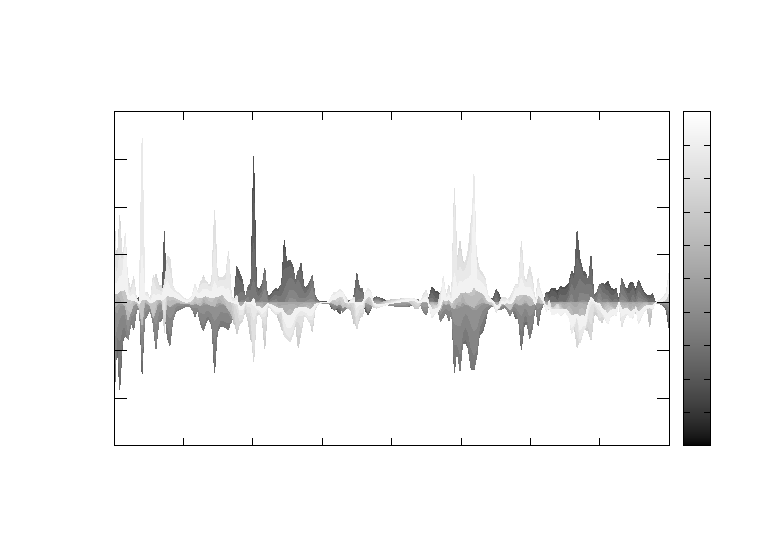
\includegraphics[width={360.00bp},height={252.00bp}]{stt-energy3d-0.3.eps}}%
    \gplfronttext
  \end{picture}%
\endgroup
}
    \caption{ A) Spin-torque plotted of borophene with the armchair edge, with $4$ unit cells width, for magnetization variable of leads with respect to the relative degree in z-direction in $E = 0\; eV$. B, C, D) Spin torque with $0.1,\;0.2,\;0.3\;eV$ magnetization respect to energy in all range of relative angles}
    \label{fig:stt}
\end{figure*}

A five-band tight-binding model with suitable hopping and on-site energy factors has been demonstrated to be in good agreement with first-principles calculations\cite{feng2017dirac}. Because of the effects of the Ag substrate, the on-site energies in this model break the structure's inversion symmetry, which is why it is known as the inversion non-symmetric (INS) model. An inversion symmetric (IS) model is constructed to eliminate substrate effects, and a homogeneous model is constructed to add homogeneity\cite{ezawa2017triplet}. All these coefficients are presented in Table\ref{tbl:hopping}.

\begin{table}[h]
\small
  \caption{The ${\beta}_{12}$-borophene hoping parameters introduced by Ezawa\cite{ezawa2017triplet}}
  \label{tbl:hopping}
  \begin{tabular*}{0.48\textwidth}{@{\extracolsep{\fill}}llllllll}
    \hline
    & H & INS & IS & & H & INS & IS \\
    \hline
    $\varepsilon_a$& 0 & 0.196 & 0.196 & $t_{ab}=t_{de}$& -2 & -2.04 & -2.04 \\
    $\varepsilon_b$& 0 & -0.058 & -0.058 & $t_{ac}=t_{ce}$& -2 & -1.79 & -1.79 \\
    $\varepsilon_c$& 0 & -0.845 & -0.845 & $t_{ae}$& -2 & -2.12 & -2.12 \\
    $\varepsilon_d$& 0 &  0.196 & -0.058 & $t_{bc}=t_{cd}$& -2 & -1.84 & -1.84 \\
    $\varepsilon_e$& 0 & -0.058 &  0.196 & $t_{bd}$& -2 & -1.91 & -1.91  \\
    \hline
  \end{tabular*}
\end{table}

As shown in Fig.\ref{fig:model}, a non-magnetic borophene nanoribbon (BNR) with two ends (as a central region) sandwiched between two semi-infinite FM borophene nanoribbons (as two electrodes) forms a spin-valve device. It is worth noting that the borophene charge carriers are generally not spin-polarized, and the magnetic property is injected into the borophene leads by an insulating ferromagnetic substrate (by growing borophene on FM insulation). Since the application of a magnetic field can be used to break the time reversal symmetry, the exchange field created through the proximity effect caused by a ferromagnetic insulating substrate, causes the time reversal or spin symmetry to be broken. Unlike alternative methods to break TRS, such as transition metal atom doping\cite{zhang2013stability,chang2013experimental} and atomic bulking\cite{feng2017experimental,yan2021newly}, this technique is an external short-range interaction manipulation that has no effect on electron mobility in electronic applications.

If the core region has a length of $L$ and contains $N$ atoms in width, this region contains $5N(2L + 1)$ atoms. The total Hamiltonian of the spin valve system is given by:
\begin{equation}
    H= H_L + H_R + H_c + H_T,
\end{equation}
Where
\begin{equation}
H_{L}=\sum\limits_{i\in L,\sigma }{\left( E_{L}+\sigma M_{L} \right)} a_{i\sigma }^{\dagger} a_{i\sigma }-\sum\limits_{i,i+\alpha \in L,\sigma}{\left( t_{\alpha } a_{i\sigma}^{\dagger} a_{i+\alpha \ \sigma }+H.c.\right)},
\end{equation}
\begin{equation}
\begin{split}
H_{R}=\sum_{i\in R,\sigma}{\left( E_{R}+\sigma M_{R} cos\phi M_{R}\sin \phi\right)} a_{i\sigma}^{\dagger} a_{i\sigma } \\
-\sum_{i\in R,\sigma} t_{\alpha } a_{i\sigma}^{\dagger} a_{i+\alpha\sigma}+H.c.,
\end{split}
\end{equation}
\begin{equation}
H_{C}=\sum_{i\in \ C,\sigma }{{{E}_{C}}}a_{i\sigma }^{\dagger}{{a}_{i\sigma }}-\sum_{i,i+\alpha \in \ C,\sigma }{({{t}_{\alpha }}\ a_{i}^{\dagger }{{a}_{i+\alpha }}+H.c.)},
\end{equation}
\begin{equation}
H_{T}=-\sum_{i\in \ C,i+\alpha \in L,R,\sigma}{{{t}_{\alpha }}}\ a_{i\sigma }^{\dagger }{{a}_{i+\alpha \ \sigma }}+H.c.,
\end{equation}
Where $E_L$, $E_R$,  and $E_C$ are the on-site energies in the borophene nanoribbons in left and right leads, and central region, respectively , which can be tuned by the gate voltage,  depending on the location of the lattice point, as shown in Table\ref{tbl:hopping}. $a^{\dagger}_{i\sigma}$($a_{i\sigma}$) are the creation (annihilation) operators of the electron at site $i$, with spin index ($\sigma$). $M_L$ and $M_R$ are the magnetizations of the left and right FM electrodes and $\theta$ is the angle between the orientations of $M_L$ and $M_R$. The electric current flowing through the system may be characterized using the non-equilibrium Green's function approach.
\begin{equation}
    I^{\sigma}=\frac{e}{h}\int{d}\varepsilon \ {{T}_{LR\sigma}}(\varepsilon )[{{f}_{L}}(\varepsilon )-{{f}_{R}}(\varepsilon )],
\end{equation}
Where $I = I^{\uparrow} + I^{\downarrow}$ and $f_{\lambda}$($\lambda=L,R$) is the Fermi distribution function for the electrode and the transmission coefficient $T(\varepsilon)$ is denoted by:
\begin{equation}
    T_{LR\sigma}(\varepsilon)=Tr [\Gamma_{L\sigma}(\varepsilon) G^{r}_{\sigma}(\varepsilon)\Gamma_{R\sigma}(\varepsilon) G^{a}_{\sigma}(\varepsilon)],
\end{equation}
With overlapping function ${{\Gamma}_{\lambda\sigma}}(\varepsilon)$  and retarded (advanced) Green function $G^{r}_{\sigma}(\varepsilon)$ defined, respectively, by:
\begin{equation}
    \Gamma_{\lambda\sigma}(\varepsilon)=i[\Sigma^{r}_{\lambda\sigma}(\varepsilon)-\Sigma^{a}_{\lambda\sigma}(\varepsilon)],
\end{equation}
\begin{equation}
    G^{r}_{\sigma}(\varepsilon )=[G^{a}(\varepsilon)]=[\frac{1}{\varepsilon}-H_{c}-\Sigma_{L\sigma}^{r}(\varepsilon)-\Sigma_{R\sigma}^{r}(\varepsilon)]^{-1},
\end{equation}
Where $\Sigma_{L\sigma(R\sigma)}$ is the left (right) lead retarded self-energy function in spin space\cite{zhou2016spin}. Note that the effect of semi-infinite electrodes on the Hamiltonian of the system is described using self-energy terms. The self-energies are calculated iteratively\cite{modarresi2011transport,norouzi2021controllable}.
% The retarded (advanced) self-energy may be calculated by the surface Green's function for the $\lambda$ electrode\cite{brey2007electronic,ding2009magnetic}. Once the electric current is determined, the conductance may be computed using $G = I/V$. For a low bias voltage, the conductance at zero temperature is given by:
Now, the total conductance for the junction can be obtained as follows:
\begin{equation}
    G(\varepsilon) =\frac{e^2}{h}\Sigma_{\sigma}T_{LR\sigma}(\varepsilon),
\end{equation}
Where $E_F$ stands for Fermi energy. According to Eq. 10, the MR may be calculated using the standard definition.
\begin{equation}
    MR = \frac{G(0)-G(\pi)}{G(0)},
\end{equation}
Where $G(0) = G(\phi= 0)$ $[G(\pi) = G(\phi=\pi)]$ is the conductance for the P(AP) configuration of the magnetizations of both electrodes.

When the magnetizations are noncollinear (the magnetizations of the left and right electrodes are neither parallel nor anti-parallel but depart from one another at an angle $\theta$), the spin-polarized current flowing through the system induces a spin torque on the right ferromagnet, which is known as CISTT\cite{slonczewski1989j}. The CISTT may be estimated by finding the temporal evolution rate of the total spin at a suitable ferromagnetic electrode. Finally, using the non-equilibrium Green's function approach, one may deduce:
\begin{equation}
\begin{split}
    \tau^{R_x}=\frac{e}{4\pi}\int{d}\varepsilon G^{r}(\varepsilon)\Gamma_{L}(\varepsilon) G^{a}(\varepsilon) \Gamma _{R}(\varepsilon)
    \times \left( {{\sigma}_{x}}cos\phi -\sigma_{z} sin\phi \right)) \\
    \left[f_{L}(\varepsilon)-f_{R}(\varepsilon)\right],
\end{split}
\end{equation}
Where $\sigma_x$ and $\sigma_z$ are the Pauli matrices. Since the nanoribbon may be considered as a periodic arrangement of unit cells in the $x$ direction, the Hamiltonian depending on $k_x$, based on the Bloch theorem, can be expressed as:
\begin{equation}
    H(k_x) = H_t e^{ik_x a} + H_0 + H_t e^{-i k_x a}.
\end{equation}

Furthermore, by diagonalizing the Hamiltonian, one can easily obtain the energy dispersion of the band structure. $H_0$ is the Hamiltonian of an arbitrary unit cell of the nanoribbon, $H_t$ is the hopping energy between two adjacent unit cells, and $a$ is the lattice constant.

\section{Result and Discussion:}
The use of two-dimensional materials, graphene and silicene, as bases for spin valves has received much attention. Borophene, as another two-dimensional material with its new properties, has been less studied for this purpose. In this article, we will also use borophene for the same purpose. Due to the numerous practical applications in devices such as switches, hard disk heads, and MRAMs, as well as STT-MRAMs, and the importance of parameters such as conductance (parallel and anti-parallel), MR, and STT in the design of a spin valve, the study of these properties in borophene will be taken into account.

The result of numerical calculations for the CPP for parallel (P) and anti-parallel (AP) configurations consisting of a nanoribbon with a width of four unit cells is shown in Fig.\ref{fig:model}. In all calculations, the left and right electrodes are considered as a borophene channel with equal magnetization, as $M_L=M_R=M$. The magnetic property is injected into the borophene leads by an insulating ferromagnetic substrate (by growing borophene on FM insulation). The angle $\theta$ determines the general orientation of the right and left leads magnetization relative to each other, while the special case $\theta=0(\pi)$ indicates the parallel (or antiparallel) magnetizations of the left and right leads, respectively.

The transmission spectra of pure borophene nanoribbon, in two different zigzag and armchair edges (BNRs), reveal a well-known step-like structure. The number of energy subbands in each energy determines the corresponding step height. Furthermore, unlike graphene nanoribbons (GNRs), the number of conduction channels in Fermi energy does not remain constant in borophene nanoribbons\cite{gmitra2016trivial}, and the number of channels grows as the width of the nanoribbons increases, which is more visible in zigzag nanoribbons than armchair nanoribbons\cite{ezawa2017triplet}. Unlike graphene, whose conductance in Fermi energy (here $E= 0\;eV$) does not depend on the width of the nanoribbon, the borophene conductance in Fermi energy changes with the change of nanoribbon width. The reason for this can be found in the difference in the number of subbands between graphene and borophene, which cross the zero Fermi energy, and this is due to the presence of an additional atom in the center of unit cell in borophene. So, it can be said that the center atom inside the unit cell in borophene accounts for the dependence of conductance channels on the width of the nanoribbon in Fermi energy. Supercells may be identified by their top and bottom edge atom names, such as ZNBR-cd, which ends in an a-c atom on the top edge and an a-d atom on the bottom edge.

Our calculations show that, despite having a very narrow band gap, the 8.8\AA\;width ZNBR-cd exhibits metallic characteristics. In many previous studies, the supercells considered in the calculations ended with one cell on both sides\cite{feng2017dirac,ezawa2017triplet}. In the current study, it has been done in the same way. Because every ABNR can terminate in b-d(ac-a), which we name $\alpha(\gamma)$, we have four types of ABNR supercells, one of which is ABNR-$\alpha\alpha$. Our calculations show that, unlike ZBNRs, ABNRs exhibit semiconducting or metallic behavior depending on the width of the ribbon $W$, so that for widths larger than a critical value $W_c = 11.08$ \AA,\cite{nikan2022effects} non-zero conductance can be found, whereas the system behaves like a semiconductor for widths smaller than $W_c$. Edge states can be observed in the energy gaps of semiconductors as well as local band gaps of conductors. As a result, even though semiconductors are typically used, zero modes can be generated at appropriately specified widths\cite{brey2006electronic}. As a result, the characteristics of armchair nanoribbons alternate between semiconductors and conductors.

Applying an in-plane exchange magnetic field causes the spin-polarized Hamiltonian not to commute with the spin operator S, and in this case, the spin of the electron will no longer be a constant of motion in the system. This implies that the spin state may change along the transport direction. Indeed, as a result of the interaction of the electron spin with the in-plane exchange magnetic field, spin rotation occurs, i.e., for example, an electron that enters the channel with a spin-up state may leave the channel as a spin-down state. 

When a magnetic field is applied to the leads due to the presence of a ferromagnetic insulating substrate, an out-of-plane magnetic field is introduced into the spin valves. According to our investigations, in this case the conductance shows changes compared to the case of non-magnetic leads. A careful analysis of these changes to understand them and know their origin is a key issue for designing applicable spin valves and exploiting their full potential.

As a result of changing the magnetic properties of the leads from non-magnetized case to the magnetized one, there is a change in the number and width of the plateaus. However, as the magnetization increases in the electrodes, deviation from the step-like structure is clearly observed. The reason for this can be described based on the exit of some energy levels from the transmission energy window due to the separation of energy levels in the electrodes, along with energy subband parity conservation as one of the other mechanisms affecting the transmission. The spin separation caused by the Zeeman Effect changes the band structure, and in an energy window, the number of subbands in both cases of magnetized and non-magnetized leads changes. In the following, we describe the deviations in conductance in magnetized leads, in comparison with non-magnetized one, which the diagrams depict the conductance for different magnetizations M and compare them with M=0 case.

One of the variations from non-magnetized lead case to the magnetized one is the change in the number and width of the plateaus in the conductance diagram, which occurs with increasing magnetization. The plateaus in the transmission diagram are seen in the range of energy where the number of subbands involved in the transmission process is constant, and when the number of subbands in each energy changes, the conductance also changes. Therefore, the width of the plateaus in the conductance diagram depends on the difference between the energy subbands. Due to the diatomic basis of materials such as graphene, silicene, etc, the indentation of the subbands does not occur even when exchange interaction is taken into account. Two types of inter-band spacing are seen; the first is the spacing between two spin subbands of the same opposite alignment, which is equal to $2M$, and the other is the spacing between the $N-1$-th spin-down band and the $N$-th spin-up subband. In borophene, due to the presence of an additional atom located in the center of the hexagon, there is an indentation of the energy levels resulting from the exchange interaction. For this reason, the diversity of the spacing between the subbands is much greater than before, which is associated with the variety of the widths of the plateaus and is also confirmed in the conduction Fig\ref{fig:conductance}.b. Therefore, the exchange interaction further changes the step-like pattern of conductance due to the variation it creates in the inter-band spacing.

One of the first deviations that can be found in magnetized leads shown in Fig\ref{fig:conductance}.a, b compared to the non-magnetized case is the presence of steps or fluctuations in conductance with values smaller than $G_0$ ($G_0 = e^2/h$) in each configuration. The cause of this phenomenon is the mismatch between the parity of the subbands of the channel and the parity of the subbands of the electrodes, whose tunnel value is less than one $G_0$ in contrast with the non-magnetic case. This means that in addition to the number of subbands in that energy window, the parity of the subbands is also very important in tunneling and electron transmission processes. This subsequently causes plateaus with odd values (which can be said to have semi-metallic properties) or semi-integer values. Of course, unlike graphene, this type of electron tunneling, which is seen in graphene only at $E_F<M$, can be seen in borophene across the whole energy spectrum. In the absence of any interactions that reduce the tunneling rate, according to the contribution $G_0$ due to each subband in the energy window (as can be seen in the P case), the presence of each plateau with a height of 2$G_0$ in the conduction diagram indicates the total rate of tunneling in the energy window. In the AP case, the full rate of tunneling does not occur in two situations: 

1. When the two subbands associated with the two electrodes have opposite parities, conduction would be zero despite the absence of an energy gap in the band structure. In the AP configuration, the numbering of the energy bands in the left and right electrodes is different from each other, and the parity of the subbands is also opposite; that is, subbands with the same numbers in two electrodes have opposite parities. In this case, based on the parity selection rule, tunneling will be prohibited, which means during the tunneling process, the electron with even parity in the left electrode cannot be converted to the electron with odd parity in the right electrode, and so despite the absence of any bandgap, the conductance will be zero. (For such an electron, even if the band gap is zero, the conduction will still be zero.)

The number of subbands depends on the number of atoms in the supercell, and in the absence of a magnetic field, they are having double spin degeneracy. In electrodes, when the magnetic substrate applies a magnetic field to the plate, splitting of the energy levels occurs. Therefore, the number of subbands is doubled. On the other hand, we know that the subbands have parity symmetry due to the symmetric structure of the $H_k$ matrix, which depends on their number; that is, the subbands 0, 2, 4, and $\dots$ are even, and the subbands 1, 3, 5, and $\dots$ are also odd. When the subbands are split, this numbering is done again from the beginning. Therefore, in the AP configuration, for example, subband 8 splits into two bands 8 up and 8 down, whose order is reversed in the opposite electrode. Due to the renumbering to parity, the subbands with the same number in two electrodes with opposite magnetizations will have opposite parity, and so tunneling does not take place in this case because electron tunneling is prohibited whenever the spins of the subbands in two electrodes are opposite to each other. That means that an even-parity electron at the left electrode will not yield an odd-parity electron at the right electrode during the tunneling process, leading to zero conductance, even in the absence of a band gap in that energy range.

2. In the situation where a parity mismatch occurs in the subbands between the electrodes and the central channel. In this case, the tunneling contribution in each subband will be less than $G_0$, and as a result, the conductance will be less than $2\;G_0$. (e.g. energy ranges $-1\;eV$ to $0.0\;eV$ for $M= 0.3\;eV$ in Fig.\ref{fig:bandconductance}.e. in some energies in the range of $-0.60\;eV$ to $-0.38\;eV$, as can be seen in the Fig.\ref{fig:conductance}.a, the conductance becomes zero for $M=0.2\;eV$. Due to the fact that the band structure diagram does not have any band gap in this range, as seen in Fig.\ref{fig:bandconductance}.a,b,c, the reason for the zero conductance can be explained based on the parity selection rules in tunneling. In fact, more precisely, in this case, the coordination between the number of subbands in this energy window and their parity is such that these conductance zeros are created. However, all conductance zeros will not necessarily result from this coordination, and this energy window is an example.

Also, in an ABNR with a P configuration containing four unit cells in width (similar to the AP configuration), the plateau width decreases, preserving the step-like structure of conductance at small magnetization. The zero conductance at energies of $-0.6\;eV$ and $0.38\;eV$ and $0.63\;eV$ to $0.83\;eV$ (for $M = 0.2\;eV$), $0.35\;eV$ to $0.56\;eV$ (for $M = 0.3\;eV$) no longer occurs. As can be seen, despite the same conditions as the P and AP configurations Fig.\ref{fig:bandconductance}.d, e (such as the type of edges, energy windows, and magnetization of the leads), the reason for the non-zero conductance in the P configuration is that, unlike the AP configuration, the parity selection rule is preserved.

Of course, it is still possible to consider semi-metallic behavior for this configuration at energies around $0.3\;eV$ (with $M = 0.3\;eV$ magnetization) and $-0.6\;eV$ (with $M = 0.2\;eV$ magnetization). The small fluctuations in the conductance Fig\ref{fig:conductance}.c,d are caused by the mismatch of the parity of the transverse wave functions in the electrodes and the channel. In this case, electron transmission takes place, but at a lower rate than in the case where the parity of the two subbands in the electrode and the channel are the same (which is one $G_0$ in our case).

Zigzag borophene nanoribbons generally show more conductance properties, which can be seen by examining their band structure and comparing it with that of armchair borophene nanoribbons. Although the fluctuations of the conductance can be observed here as well, which are caused by the mismatch of the parity of the states in the electrodes and the channel, the conductance does not show many changes with the increase in magnetization. Also, zero conductance does not appear. The difference between the P and AP configurations in zigzag borophene is much less than in armchair borophene, which subsequently should lead to the conclusion that zigzag borophene will be less valuable in the spin valve device.

Examining MR provides an important criterion for the possibility of using a device as an appropriate spin valve. This means that if a device has a high magnetoresistance in addition to having significant changes in conductance between P and AP configurations, it can be a good potential candidate for a spin valve device. According to the definition of MR, it is obvious that its value must be zero for $M = 0\;eV$, because in this case, there is no difference between AP and P configurations. In fact, the non-zero values of $M$ distinguish the two configurations mentioned from each other. As can be seen in Fig\ref{fig:MR}.a when $M=0.05\;eV$, a perfect plateau structure can be observed. In this case, the A-configure is a non-conductor with zero conductance, whereas the P-configure shows good conductance properties with about a $G_0$ value.

We know that when there are plateaus of $100\%$ in the MR diagram, the conductance in the AP becomes zero, and the conductance is large enough for the P-configuration, which is apparent from Fig\ref{fig:MR}.b, which is about one $G_0$. Compared to graphene and silicene, the MR peaks in borophene are much more irregular and less histogram-like, as depicted in Fig\ref{fig:MR}.a. For $M = 0.05\;eV$, a $100\%$ plateau (perfect plateau) occurs at an energy of $3.8\;eV$ where the width of the plateau increases with rising $M$ to $0.1\;eV$. Which is consistent with our knowledge of the variation of plateau width with $M$. As can be seen in Fig.\ref{fig:conductance}.a, the number of energy windows with zero conductance in the AP configuration is much higher at $M = 0.2\;eV$ and $M = 0.3\;eV$, and therefore the number of $100\%$ plateaus is also higher. 

Unlike graphene and other 2D materials, where $100\%$ of the plateaus (perfect plateau) are located around the Dirac point energy $E_F = 0\;eV$, in borophene, $100\%$ of the plateaus occur at all energies and show a lower histogram shape. This phenomenon can be considered an advantage for borophene because the application of graphene magnetoresistance in switching is limited to specific energy (Dirac point energy), while there is no such limitation for borophene. It means that there are more choices in the energy range to set other parameters that are necessary for making devices, and we are not limited to a specific energy. 

The variation of $100\%$ plateau widths in borophene is primarily due to the zero AP conductance, which is subsequently obtained based on the spacing of the subbands and the parity selection rule, as stated in the previous sections. As it is clear, as the conductance has zeros with a larger width (that is, the conductance is zero in a larger energy range), the same energy widths with zero conductance are reflected in the MR diagram with plateaus with a value of one. Therefore, the description of the plateau width of the MR diagram depends entirely depends on the two factors that determine the conductance zeros.

The cause of the valleys in the MR diagram is attributed to the smaller spacing between the subbands in each magnetization, which leads to the conduction in the two configurations being close to each other. As a result, it can be concluded that the conductance at those points is somewhat independent of the orientation of the electrodes.

The next generation of spin valves is the modified one based on spin transfer torque (STT), which is promising because of its potential in non-volatile memory with near-zero leakage power consumption and offering opportunities to supplement or replace CMOS-based Boolean logic, and hence, it deserves further investigation and attention. Spin-polarized electrons flowing from the left to the right FM electrode may produce a torque called a spin transfer torque (STT) if the magnetization is deflected by an angle to the left. In general, STT is a vector that can be split into in-plane and out-of-plane components using small bias voltages. The latter is very small and could be ignored.

The variation of torque with $\theta$, as shown in Fig.\ref{fig:stt}.a, can be fitted with a good approximation by a model including the first two harmonics presented below, with the parameters shown in the Table\ref{tbl:fitting} Fitting the STT-$\theta$ plot with $a\sin(\theta)+b\sin(2\theta)+c$. Moreover, as $M$ increases, $\tau_x/V$ increases too, which confirms that $\tau_x/V$ is proportional to the polarization of the FMs.

As predicted, the torque exhibits an oscillation-like behavior, consistent with previous numerical simulations for graphene\cite{maher2022spin}, silicene\cite{cheraghchi2012edge},and quantum dot\cite{pham2020electronic}. This is because the STT is proportional to $M_R\times (M_L\times M_R)$, resulting in a sin $\theta$ factor. Hence, the torque vanishes with collinear alignment $(\theta = 0,\pi)$ of the two FMs and vanishes completely with $M = 0\;eV$ (not illustrated here). It appears that the oscillation-like behavior is actually a sinusoidal behavior with more harmonics in borophene, as opposed to graphene and silicene, which have a purely sinusoidal behavior.
In this curve, the maximum value of spin torque is obtained in the relative direction of $61^\circ$ when the magnetization of the electrodes is $0.1\;eV$. On the other hand, as the spin magnetization in the electrodes increases, the value of the spin torque decreases. There is also a rotational symmetry around the axis.

The plot of STT versus Fermi energy and relative angles of the electrodes is presented in Fig.\ref{fig:stt}.b. As expected, the graph shows peaks that are proportional to the difference between spin-up and spin-down transmissions. The larger the difference, the sharper peaks are seen, and the points with near-zero STT indicate that the difference between up and down spin transmission is very small. 

In graphene and silicene, the peaks become sharper as one moves away from $E_F = 0\;eV$, which is due to both spin transport oscillations near the Fermi energy and step-like behavior in regions far from the Fermi energy. However, this is not observed in borophene due to the indentation of the subbands. The spin transport in borophene exhibits oscillatory and step-like behaviors simultaneously in different regions. Therefore, the STT peaks, which are calculated based on the difference in the transmission of the up and down spins, show the same behavior; furthermore, long and short peaks are seen in the entire energy range.

Although the order in the STT curve of graphene may not be seen in borophene, since one of the applications of spin valve devices is the separation of spins, this diversity and dispersion of peaks provide more possibilities for controlling the spin separation.

The ability to transfer spin information can enable sophisticated spintronic devices, such as reconfigurable logic gates that integrate memory and logic, paving the way for spin information processing. However  many parameters such as injection and detection and spin propagation length must be simultaneously significant and improved to be effective in the design and fabrication of complex spintronic devices, the existence of energies at which the spins up and down have different energy spectrums is a necessary condition for the operation of the device\cite{seneor2012spintronics, zhou2016spin}.

Therefore, the presence of more peaks in an energy range in the STT diagram indicates the energies at which the up and down spins are separated from each other. As we said, to use a system in the manufacture and design of spintronic devices, many conditions must be determined, each of which may depend on energy. Therefore, the presence of peaks indicating spin separation at different energies can be used in system control to select the most optimal energy point in order to expand the study or design of manufacturing spintronic devices.

\section{Conclusion:}
\begin{table}[t]
\small
  \caption{\ Fitting parameter for STT vs $\theta$}
  \label{tbl:fitting}
  \begin{tabular*}{0.48\textwidth}{@{\extracolsep{\fill}}llll}
    \hline
    M(eV) & a & b & c \\
    \hline
    0.3 & -0.0649309 & 0.0726612 & 2.52642e-05 \\
    0.2 & 0.00900465 & 0.0655489 & -3.70375e-05 \\
    0.2 & 0.205575 & 0.0879828 & -0.00388147 \\
    0.05 & 0.200799 & 0.0728197 & -0.00673132 \\
    \hline
  \end{tabular*}
\end{table}
In conclusion, the research presented in this article explores the potential of borophene as a base material for spin valves in spintronics. The advantages of borophene compared to other two-dimensional materials are highlighted, including its unique properties such as low density, high hardness, heat resistance, and electrical conductance.

The theoretical analysis of spin-dependent transport and spin transfer torque in borophene-based FM/normal/FM junctions reveals promising results, including perfect magnetoresistance plateaus in all ranges of energies, conductance gap in AP configuration without band gap due to parity selection rule, MR perfect plateaus not only occur in around Dirac point energy (like graphene and silicene, etc.) but also occur in all energies ranges that resolve limitations of specific energies to work, a sinusoidal oscillatory pattern in spin transfer torque, and more diversity and dispersion of STT-E curve peaks to more possibilities for controlling the spin separation. These calculated results demonstrate the potential of borophene as a promising material for spin valve devices in spintronics.

One of the key findings is the observation of perfect magnetoresistance plateaus in borophene, indicating its potential as an excellent spin valve candidate. The conductance diagram shows more zeros in the anti-parallel configuration, allowing for more precise control of the device in creating ON and OFF modes for switching. This feature makes borophene an excellent candidate for spin valves. Additionally, the sinusoidal oscillatory pattern in the spin transfer torque (STT) at different relative angles between the magnetic electrodes amplifies as the magnetic intensity increases, providing a means for manipulating the spin in the device. 

Comparisons with other two-dimensional materials such as graphene and silicene demonstrate the unique behavior of borophene in terms of conductance and STT. The STT in borophene shows a sinusoidal behavior with more harmonics compared to other materials.

Furthermore, the plot of STT versus Fermi energy and the relative angles of the electrodes demonstrates peaks that are proportional to the difference between spin-up and spin-down transmission. The sharpness of the peaks indicates a larger difference in transmission, while near-zero STT points indicate a very small difference. The STT also depends on the relative angle between the electrodes, with zero STT observed at angles that are multiples of $\theta$. Overall, the research on borophene-based spin valves provides valuable insights into the potential of this material in spintronics. The unique properties and behavior of borophene make it a promising candidate for future spin valve devices. Further exploration and development in this field will contribute to the advancement of spintronics technology and its applications in non-volatile memory and logic devices.

\section*{Author Contributions}
Erfan Nikan:Investigate, Validation, Software, Programming, Writing - original draft, Writing -review, editing, Resources.
Amirhossein Ahmadkhan Kordbacheh: Supervision, Project administration, Writing - review, editing, Investigation.
\section*{Conflicts of interest}
There are no conflicts to declare.
\section*{Acknowledgements}
The computing facilities of Materials Simulation Laboratory, at Department of Physics, Iran University of Science and Technology (IUST) were used.
%%%END OF MAIN TEXT%%%

%The \balance command can be used to balance the columns on the final page if desired. It should be placed anywhere within the first column of the last page.

\balance

%If notes are included in your references you can change the title from 'References' to 'Notes and references' using the following command:
%\renewcommand\refname{Notes and references}

%%%REFERENCES%%%
\bibliography{rsc} %You need to replace "rsc" on this line with the name of your .bib file
\bibliographystyle{rsc} %the RSC's .bst file

\end{document}